\documentclass[twoside]{book}

% Packages required by doxygen
\usepackage{fixltx2e}
\usepackage{calc}
\usepackage{doxygen}
\usepackage[export]{adjustbox} % also loads graphicx
\usepackage{graphicx}
\usepackage[utf8]{inputenc}
\usepackage{makeidx}
\usepackage{multicol}
\usepackage{multirow}
\PassOptionsToPackage{warn}{textcomp}
\usepackage{textcomp}
\usepackage[nointegrals]{wasysym}
\usepackage[table]{xcolor}

% Font selection
\usepackage[T1]{fontenc}
\usepackage[scaled=.90]{helvet}
\usepackage{courier}
\usepackage{amssymb}
\usepackage{sectsty}
\renewcommand{\familydefault}{\sfdefault}
\allsectionsfont{%
  \fontseries{bc}\selectfont%
  \color{darkgray}%
}
\renewcommand{\DoxyLabelFont}{%
  \fontseries{bc}\selectfont%
  \color{darkgray}%
}
\newcommand{\+}{\discretionary{\mbox{\scriptsize$\hookleftarrow$}}{}{}}

% Page & text layout
\usepackage{geometry}
\geometry{%
  a4paper,%
  top=2.5cm,%
  bottom=2.5cm,%
  left=2.5cm,%
  right=2.5cm%
}
\tolerance=750
\hfuzz=15pt
\hbadness=750
\setlength{\emergencystretch}{15pt}
\setlength{\parindent}{0cm}
\setlength{\parskip}{3ex plus 2ex minus 2ex}
\makeatletter
\renewcommand{\paragraph}{%
  \@startsection{paragraph}{4}{0ex}{-1.0ex}{1.0ex}{%
    \normalfont\normalsize\bfseries\SS@parafont%
  }%
}
\renewcommand{\subparagraph}{%
  \@startsection{subparagraph}{5}{0ex}{-1.0ex}{1.0ex}{%
    \normalfont\normalsize\bfseries\SS@subparafont%
  }%
}
\makeatother

% Headers & footers
\usepackage{fancyhdr}
\pagestyle{fancyplain}
\fancyhead[LE]{\fancyplain{}{\bfseries\thepage}}
\fancyhead[CE]{\fancyplain{}{}}
\fancyhead[RE]{\fancyplain{}{\bfseries\leftmark}}
\fancyhead[LO]{\fancyplain{}{\bfseries\rightmark}}
\fancyhead[CO]{\fancyplain{}{}}
\fancyhead[RO]{\fancyplain{}{\bfseries\thepage}}
\fancyfoot[LE]{\fancyplain{}{}}
\fancyfoot[CE]{\fancyplain{}{}}
\fancyfoot[RE]{\fancyplain{}{\bfseries\scriptsize Generated by Doxygen }}
\fancyfoot[LO]{\fancyplain{}{\bfseries\scriptsize Generated by Doxygen }}
\fancyfoot[CO]{\fancyplain{}{}}
\fancyfoot[RO]{\fancyplain{}{}}
\renewcommand{\footrulewidth}{0.4pt}
\renewcommand{\chaptermark}[1]{%
  \markboth{#1}{}%
}
\renewcommand{\sectionmark}[1]{%
  \markright{\thesection\ #1}%
}

% Indices & bibliography
\usepackage{natbib}
\usepackage[titles]{tocloft}
\setcounter{tocdepth}{3}
\setcounter{secnumdepth}{5}
\makeindex

% Hyperlinks (required, but should be loaded last)
\usepackage{ifpdf}
\ifpdf
  \usepackage[pdftex,pagebackref=true]{hyperref}
\else
  \usepackage[ps2pdf,pagebackref=true]{hyperref}
\fi
\hypersetup{%
  colorlinks=true,%
  linkcolor=blue,%
  citecolor=blue,%
  unicode%
}

% Custom commands
\newcommand{\clearemptydoublepage}{%
  \newpage{\pagestyle{empty}\cleardoublepage}%
}

\usepackage{caption}
\captionsetup{labelsep=space,justification=centering,font={bf},singlelinecheck=off,skip=4pt,position=top}

%===== C O N T E N T S =====

\begin{document}

% Titlepage & ToC
\hypersetup{pageanchor=false,
             bookmarksnumbered=true,
             pdfencoding=unicode
            }
\pagenumbering{alph}
\begin{titlepage}
\vspace*{7cm}
\begin{center}%
{\Large My Project }\\
\vspace*{1cm}
{\large Generated by Doxygen 1.8.14}\\
\end{center}
\end{titlepage}
\clearemptydoublepage
\pagenumbering{roman}
\tableofcontents
\clearemptydoublepage
\pagenumbering{arabic}
\hypersetup{pageanchor=true}

%--- Begin generated contents ---
\chapter{Namespace Index}
\section{Namespace List}
Here is a list of all documented namespaces with brief descriptions\+:\begin{DoxyCompactList}
\item\contentsline{section}{\mbox{\hyperlink{namespacesimlib_1_1action}{simlib.\+action}} }{\pageref{namespacesimlib_1_1action}}{}
\item\contentsline{section}{\mbox{\hyperlink{namespacesimlib_1_1archspec}{simlib.\+archspec}} }{\pageref{namespacesimlib_1_1archspec}}{}
\item\contentsline{section}{\mbox{\hyperlink{namespacesimlib_1_1simulated}{simlib.\+simulated}} }{\pageref{namespacesimlib_1_1simulated}}{}
\end{DoxyCompactList}

\chapter{Hierarchical Index}
\section{Class Hierarchy}
This inheritance list is sorted roughly, but not completely, alphabetically\+:\begin{DoxyCompactList}
\item \contentsline{section}{simlib.\+action.\+Action}{\pageref{classsimlib_1_1action_1_1_action}}{}
\item \contentsline{section}{simlib.\+simulated.\+Action\+Queue}{\pageref{classsimlib_1_1simulated_1_1_action_queue}}{}
\item \contentsline{section}{simlib.\+archspec.\+Arch\+Spec}{\pageref{classsimlib_1_1archspec_1_1_arch_spec}}{}
\item \contentsline{section}{simlib.\+simulationenvironment.\+Simulation\+Environment}{\pageref{classsimlib_1_1simulationenvironment_1_1_simulation_environment}}{}
\item \contentsline{section}{simlib.\+F\+S\+M.\+State}{\pageref{classsimlib_1_1_f_s_m_1_1_state}}{}
\item A\+BC\begin{DoxyCompactList}
\item \contentsline{section}{simlib.\+anchor.\+Anchor}{\pageref{classsimlib_1_1anchor_1_1_anchor}}{}
\begin{DoxyCompactList}
\item \contentsline{section}{simlib.\+D\+W1000\+\_\+\+Anchor\+\_\+1.\+D\+W1000\+\_\+\+Anchor\+\_\+1}{\pageref{classsimlib_1_1_d_w1000___anchor__1_1_1_d_w1000___anchor__1}}{}
\end{DoxyCompactList}
\item \contentsline{section}{simlib.\+F\+S\+M.\+Device}{\pageref{classsimlib_1_1_f_s_m_1_1_device}}{}
\begin{DoxyCompactList}
\item \contentsline{section}{simlib.\+anchor.\+Anchor}{\pageref{classsimlib_1_1anchor_1_1_anchor}}{}
\item \contentsline{section}{simlib.\+F\+S\+M.\+D\+W1000}{\pageref{classsimlib_1_1_f_s_m_1_1_d_w1000}}{}
\item \contentsline{section}{simlib.\+node.\+Node}{\pageref{classsimlib_1_1node_1_1_node}}{}
\begin{DoxyCompactList}
\item \contentsline{section}{simlib.\+D\+W1000\+\_\+\+Node\+\_\+1.\+D\+W1000\+\_\+\+Node\+\_\+1}{\pageref{classsimlib_1_1_d_w1000___node__1_1_1_d_w1000___node__1}}{}
\end{DoxyCompactList}
\end{DoxyCompactList}
\item \contentsline{section}{simlib.\+hub.\+Hub}{\pageref{classsimlib_1_1hub_1_1_hub}}{}
\begin{DoxyCompactList}
\item \contentsline{section}{simlib.\+Example\+Hub.\+Example\+Hub}{\pageref{classsimlib_1_1_example_hub_1_1_example_hub}}{}
\end{DoxyCompactList}
\item \contentsline{section}{simlib.\+simulated.\+Simulated}{\pageref{classsimlib_1_1simulated_1_1_simulated}}{}
\begin{DoxyCompactList}
\item \contentsline{section}{simlib.\+archspec.\+My\+Subclass}{\pageref{classsimlib_1_1archspec_1_1_my_subclass}}{}
\item \contentsline{section}{simlib.\+F\+S\+M.\+Device}{\pageref{classsimlib_1_1_f_s_m_1_1_device}}{}
\item \contentsline{section}{simlib.\+hub.\+Hub}{\pageref{classsimlib_1_1hub_1_1_hub}}{}
\end{DoxyCompactList}
\end{DoxyCompactList}
\end{DoxyCompactList}

\chapter{Class Index}
\section{Class List}
Here are the classes, structs, unions and interfaces with brief descriptions\+:\begin{DoxyCompactList}
\item\contentsline{section}{\mbox{\hyperlink{classsimlib_1_1action_1_1_action}{simlib.\+action.\+Action}} \\*Classes \#\# }{\pageref{classsimlib_1_1action_1_1_action}}{}
\item\contentsline{section}{\mbox{\hyperlink{classsimlib_1_1simulated_1_1_action_queue}{simlib.\+simulated.\+Action\+Queue}} }{\pageref{classsimlib_1_1simulated_1_1_action_queue}}{}
\item\contentsline{section}{\mbox{\hyperlink{classsimlib_1_1anchor_1_1_anchor}{simlib.\+anchor.\+Anchor}} }{\pageref{classsimlib_1_1anchor_1_1_anchor}}{}
\item\contentsline{section}{\mbox{\hyperlink{classsimlib_1_1archspec_1_1_arch_spec}{simlib.\+archspec.\+Arch\+Spec}} \\*Classes \#\# }{\pageref{classsimlib_1_1archspec_1_1_arch_spec}}{}
\item\contentsline{section}{\mbox{\hyperlink{classsimlib_1_1_f_s_m_1_1_device}{simlib.\+F\+S\+M.\+Device}} }{\pageref{classsimlib_1_1_f_s_m_1_1_device}}{}
\item\contentsline{section}{\mbox{\hyperlink{classsimlib_1_1_f_s_m_1_1_d_w1000}{simlib.\+F\+S\+M.\+D\+W1000}} }{\pageref{classsimlib_1_1_f_s_m_1_1_d_w1000}}{}
\item\contentsline{section}{\mbox{\hyperlink{classsimlib_1_1hub_1_1_hub}{simlib.\+hub.\+Hub}} }{\pageref{classsimlib_1_1hub_1_1_hub}}{}
\item\contentsline{section}{\mbox{\hyperlink{classsimlib_1_1archspec_1_1_my_subclass}{simlib.\+archspec.\+My\+Subclass}} }{\pageref{classsimlib_1_1archspec_1_1_my_subclass}}{}
\item\contentsline{section}{\mbox{\hyperlink{classsimlib_1_1node_1_1_node}{simlib.\+node.\+Node}} }{\pageref{classsimlib_1_1node_1_1_node}}{}
\item\contentsline{section}{\mbox{\hyperlink{classsimlib_1_1simulated_1_1_simulated}{simlib.\+simulated.\+Simulated}} \\*Classes \#\# }{\pageref{classsimlib_1_1simulated_1_1_simulated}}{}
\item\contentsline{section}{\mbox{\hyperlink{classsimlib_1_1simulationenvironment_1_1_simulation_environment}{simlib.\+simulationenvironment.\+Simulation\+Environment}} }{\pageref{classsimlib_1_1simulationenvironment_1_1_simulation_environment}}{}
\item\contentsline{section}{\mbox{\hyperlink{classsimlib_1_1_f_s_m_1_1_state}{simlib.\+F\+S\+M.\+State}} }{\pageref{classsimlib_1_1_f_s_m_1_1_state}}{}
\end{DoxyCompactList}

\chapter{Namespace Documentation}
\hypertarget{namespacesimlib_1_1action}{}\section{simlib.\+action Namespace Reference}
\label{namespacesimlib_1_1action}\index{simlib.\+action@{simlib.\+action}}
\subsection*{Classes}
\begin{DoxyCompactItemize}
\item 
class \mbox{\hyperlink{classsimlib_1_1action_1_1_action}{Action}}
\begin{DoxyCompactList}\small\item\em Classes \#\#. \end{DoxyCompactList}\end{DoxyCompactItemize}
\subsection*{Functions}
\begin{DoxyCompactItemize}
\item 
\mbox{\Hypertarget{namespacesimlib_1_1action_ab7fe3c0b13e6245919ae875f53e402a2}\label{namespacesimlib_1_1action_ab7fe3c0b13e6245919ae875f53e402a2}} 
def {\bfseries fn} (n)
\item 
\mbox{\Hypertarget{namespacesimlib_1_1action_a04debf992e34c2c78decde32950215f8}\label{namespacesimlib_1_1action_a04debf992e34c2c78decde32950215f8}} 
def {\bfseries fn2} (x, y)
\end{DoxyCompactItemize}
\subsection*{Variables}
\begin{DoxyCompactItemize}
\item 
\mbox{\Hypertarget{namespacesimlib_1_1action_a7c9b53dfdf7b83201f3b579c0babbaa0}\label{namespacesimlib_1_1action_a7c9b53dfdf7b83201f3b579c0babbaa0}} 
int {\bfseries errors} = 0
\item 
\mbox{\Hypertarget{namespacesimlib_1_1action_a0b9adc670ea622af1a4ac000c4551503}\label{namespacesimlib_1_1action_a0b9adc670ea622af1a4ac000c4551503}} 
{\bfseries test\+\_\+obj} = None
\end{DoxyCompactItemize}


\subsection{Detailed Description}
\begin{DoxyVerb}@package Action
This module defines the Action object, which is used, together with the ActionQueue class,
to implement delayed function calls.
\end{DoxyVerb}
 
\hypertarget{namespacesimlib_1_1archspec}{}\section{simlib.\+archspec Namespace Reference}
\label{namespacesimlib_1_1archspec}\index{simlib.\+archspec@{simlib.\+archspec}}
\subsection*{Classes}
\begin{DoxyCompactItemize}
\item 
class \mbox{\hyperlink{classsimlib_1_1archspec_1_1_arch_spec}{Arch\+Spec}}
\begin{DoxyCompactList}\small\item\em Classes \#\#. \end{DoxyCompactList}\item 
class \mbox{\hyperlink{classsimlib_1_1archspec_1_1_my_subclass}{My\+Subclass}}
\end{DoxyCompactItemize}
\subsection*{Variables}
\begin{DoxyCompactItemize}
\item 
int \mbox{\hyperlink{namespacesimlib_1_1archspec_a417dd2991c99643d042aec6e1c95039d}{errors}} = 0
\item 
\mbox{\hyperlink{namespacesimlib_1_1archspec_a27bb5093b53649de1394d2ba20db9a51}{archspec\+\_\+obj}} = \mbox{\hyperlink{classsimlib_1_1archspec_1_1_arch_spec}{Arch\+Spec}}( int , int , int )
\end{DoxyCompactItemize}


\subsection{Detailed Description}
\begin{DoxyVerb}@package Architecture Specification
This module presents the simulation environment with the types of the hub, nodes, and
anchors.
\end{DoxyVerb}
 

\subsection{Variable Documentation}
\mbox{\Hypertarget{namespacesimlib_1_1archspec_a27bb5093b53649de1394d2ba20db9a51}\label{namespacesimlib_1_1archspec_a27bb5093b53649de1394d2ba20db9a51}} 
\index{simlib\+::archspec@{simlib\+::archspec}!archspec\+\_\+obj@{archspec\+\_\+obj}}
\index{archspec\+\_\+obj@{archspec\+\_\+obj}!simlib\+::archspec@{simlib\+::archspec}}
\subsubsection{\texorpdfstring{archspec\+\_\+obj}{archspec\_obj}}
{\footnotesize\ttfamily simlib.\+archspec.\+archspec\+\_\+obj = \mbox{\hyperlink{classsimlib_1_1archspec_1_1_arch_spec}{Arch\+Spec}}( int , int , int )}

\mbox{\Hypertarget{namespacesimlib_1_1archspec_a417dd2991c99643d042aec6e1c95039d}\label{namespacesimlib_1_1archspec_a417dd2991c99643d042aec6e1c95039d}} 
\index{simlib\+::archspec@{simlib\+::archspec}!errors@{errors}}
\index{errors@{errors}!simlib\+::archspec@{simlib\+::archspec}}
\subsubsection{\texorpdfstring{errors}{errors}}
{\footnotesize\ttfamily int simlib.\+archspec.\+errors = 0}


\hypertarget{namespacesimlib_1_1simulated}{}\section{simlib.\+simulated Namespace Reference}
\label{namespacesimlib_1_1simulated}\index{simlib.\+simulated@{simlib.\+simulated}}
\subsection*{Classes}
\begin{DoxyCompactItemize}
\item 
class \mbox{\hyperlink{classsimlib_1_1simulated_1_1_action_queue}{Action\+Queue}}
\item 
class \mbox{\hyperlink{classsimlib_1_1simulated_1_1_simulated}{Simulated}}
\begin{DoxyCompactList}\small\item\em Classes \#\#. \end{DoxyCompactList}\end{DoxyCompactItemize}
\subsection*{Variables}
\begin{DoxyCompactItemize}
\item 
\mbox{\Hypertarget{namespacesimlib_1_1simulated_a869c9cd35f4300c21611c3493a502d2b}\label{namespacesimlib_1_1simulated_a869c9cd35f4300c21611c3493a502d2b}} 
bool {\bfseries D\+E\+B\+UG} = True
\item 
\mbox{\Hypertarget{namespacesimlib_1_1simulated_a61b1e354d4de5ca84c3ef59b995f1d94}\label{namespacesimlib_1_1simulated_a61b1e354d4de5ca84c3ef59b995f1d94}} 
int {\bfseries errors} = 0
\item 
\mbox{\Hypertarget{namespacesimlib_1_1simulated_a568d0a51b773f62750b4f5f3be304e06}\label{namespacesimlib_1_1simulated_a568d0a51b773f62750b4f5f3be304e06}} 
{\bfseries aq} = \mbox{\hyperlink{classsimlib_1_1simulated_1_1_action_queue}{Action\+Queue}}( )
\item 
\mbox{\Hypertarget{namespacesimlib_1_1simulated_a2824112ce8253f4840a2f4e50bf6d08d}\label{namespacesimlib_1_1simulated_a2824112ce8253f4840a2f4e50bf6d08d}} 
{\bfseries action1} = \mbox{\hyperlink{classsimlib_1_1action_1_1_action}{Action}}( aq.\+test, \mbox{[}\char`\"{}I was the first action added\char`\"{}\mbox{]} )
\item 
\mbox{\Hypertarget{namespacesimlib_1_1simulated_a89b7aff90a7c400753f78d0544a57f9a}\label{namespacesimlib_1_1simulated_a89b7aff90a7c400753f78d0544a57f9a}} 
{\bfseries action2} = \mbox{\hyperlink{classsimlib_1_1action_1_1_action}{Action}}( aq.\+test, \mbox{[}\char`\"{}then me (\+:\char`\"{}\mbox{]} )
\item 
\mbox{\Hypertarget{namespacesimlib_1_1simulated_accf462e21b425ff2fa68976fc5524bca}\label{namespacesimlib_1_1simulated_accf462e21b425ff2fa68976fc5524bca}} 
{\bfseries action3} = \mbox{\hyperlink{classsimlib_1_1action_1_1_action}{Action}}( aq.\+test, \mbox{[}\char`\"{}lastly me (;\char`\"{}\mbox{]} )
\item 
\mbox{\Hypertarget{namespacesimlib_1_1simulated_a043c73724dd23fd70be661f0357bb1cf}\label{namespacesimlib_1_1simulated_a043c73724dd23fd70be661f0357bb1cf}} 
int {\bfseries i} = 0
\end{DoxyCompactItemize}


\subsection{Detailed Description}
\begin{DoxyVerb}@package Simulated 
The simulated module contains the Simulated class that is an abstract class
that generalizes the notions fo a device, central hub, anchor and node. It 
also contains the ActionQueue class that is resposuble for keeping track of
the current stated of the actions that are waiting to be executed (time until
execution).
\end{DoxyVerb}
 
\chapter{Class Documentation}
\hypertarget{classsimlib_1_1action_1_1_action}{}\section{simlib.\+action.\+Action Class Reference}
\label{classsimlib_1_1action_1_1_action}\index{simlib.\+action.\+Action@{simlib.\+action.\+Action}}


Classes \#\#.  


\subsection*{Public Member Functions}
\begin{DoxyCompactItemize}
\item 
def \mbox{\hyperlink{classsimlib_1_1action_1_1_action_a9f85fbf1e0a4249eb884a10408e61583}{\+\_\+\+\_\+init\+\_\+\+\_\+}}
\item 
def \mbox{\hyperlink{classsimlib_1_1action_1_1_action_ade5a713fac538d1c6c2db749e45368d4}{decrement}}
\item 
def \mbox{\hyperlink{classsimlib_1_1action_1_1_action_a7208f5d6452283fe610143e5b0786f2b}{set\+\_\+fn}}
\item 
def \mbox{\hyperlink{classsimlib_1_1action_1_1_action_a5043b6debec6f1486a449b0393351353}{set\+\_\+ctr}}
\item 
def \mbox{\hyperlink{classsimlib_1_1action_1_1_action_ab9a687eb0392442ddf3ea24216115eab}{get\+\_\+fn}} (self)
\item 
def \mbox{\hyperlink{classsimlib_1_1action_1_1_action_a50ced713bcfa576f7177455b4b1d6d33}{get\+\_\+args}} (self)
\item 
def \mbox{\hyperlink{classsimlib_1_1action_1_1_action_a9d3d09c4547aa4bb649f1ccc168ebd3b}{get\+\_\+ctr}} (self)
\end{DoxyCompactItemize}


\subsection{Detailed Description}
Classes \#\#. 

\begin{DoxyVerb}Element of an action queue
\end{DoxyVerb}
 

\subsection{Constructor \& Destructor Documentation}
\mbox{\Hypertarget{classsimlib_1_1action_1_1_action_a9f85fbf1e0a4249eb884a10408e61583}\label{classsimlib_1_1action_1_1_action_a9f85fbf1e0a4249eb884a10408e61583}} 
\index{simlib\+::action\+::\+Action@{simlib\+::action\+::\+Action}!\+\_\+\+\_\+init\+\_\+\+\_\+@{\+\_\+\+\_\+init\+\_\+\+\_\+}}
\index{\+\_\+\+\_\+init\+\_\+\+\_\+@{\+\_\+\+\_\+init\+\_\+\+\_\+}!simlib\+::action\+::\+Action@{simlib\+::action\+::\+Action}}
\subsubsection{\texorpdfstring{\+\_\+\+\_\+init\+\_\+\+\_\+()}{\_\_init\_\_()}}
{\footnotesize\ttfamily def simlib.\+action.\+Action.\+\_\+\+\_\+init\+\_\+\+\_\+ (\begin{DoxyParamCaption}\item[{}]{self,  }\item[{}]{fn\+\_\+to\+\_\+be\+\_\+called }\end{DoxyParamCaption})}



\subsection{Member Function Documentation}
\mbox{\Hypertarget{classsimlib_1_1action_1_1_action_ade5a713fac538d1c6c2db749e45368d4}\label{classsimlib_1_1action_1_1_action_ade5a713fac538d1c6c2db749e45368d4}} 
\index{simlib\+::action\+::\+Action@{simlib\+::action\+::\+Action}!decrement@{decrement}}
\index{decrement@{decrement}!simlib\+::action\+::\+Action@{simlib\+::action\+::\+Action}}
\subsubsection{\texorpdfstring{decrement()}{decrement()}}
{\footnotesize\ttfamily def simlib.\+action.\+Action.\+decrement (\begin{DoxyParamCaption}\item[{}]{self,  }\item[{}]{n }\end{DoxyParamCaption})}

\mbox{\Hypertarget{classsimlib_1_1action_1_1_action_a50ced713bcfa576f7177455b4b1d6d33}\label{classsimlib_1_1action_1_1_action_a50ced713bcfa576f7177455b4b1d6d33}} 
\index{simlib\+::action\+::\+Action@{simlib\+::action\+::\+Action}!get\+\_\+args@{get\+\_\+args}}
\index{get\+\_\+args@{get\+\_\+args}!simlib\+::action\+::\+Action@{simlib\+::action\+::\+Action}}
\subsubsection{\texorpdfstring{get\+\_\+args()}{get\_args()}}
{\footnotesize\ttfamily def simlib.\+action.\+Action.\+get\+\_\+args (\begin{DoxyParamCaption}\item[{}]{self,  }\item[{}]{list }\end{DoxyParamCaption})}

\begin{DoxyVerb}Returns the function args associated with this action.
\end{DoxyVerb}
 \mbox{\Hypertarget{classsimlib_1_1action_1_1_action_a9d3d09c4547aa4bb649f1ccc168ebd3b}\label{classsimlib_1_1action_1_1_action_a9d3d09c4547aa4bb649f1ccc168ebd3b}} 
\index{simlib\+::action\+::\+Action@{simlib\+::action\+::\+Action}!get\+\_\+ctr@{get\+\_\+ctr}}
\index{get\+\_\+ctr@{get\+\_\+ctr}!simlib\+::action\+::\+Action@{simlib\+::action\+::\+Action}}
\subsubsection{\texorpdfstring{get\+\_\+ctr()}{get\_ctr()}}
{\footnotesize\ttfamily def simlib.\+action.\+Action.\+get\+\_\+ctr (\begin{DoxyParamCaption}\item[{}]{self,  }\item[{}]{int }\end{DoxyParamCaption})}

\begin{DoxyVerb}Returns the counter value associated with this action.
\end{DoxyVerb}
 \mbox{\Hypertarget{classsimlib_1_1action_1_1_action_ab9a687eb0392442ddf3ea24216115eab}\label{classsimlib_1_1action_1_1_action_ab9a687eb0392442ddf3ea24216115eab}} 
\index{simlib\+::action\+::\+Action@{simlib\+::action\+::\+Action}!get\+\_\+fn@{get\+\_\+fn}}
\index{get\+\_\+fn@{get\+\_\+fn}!simlib\+::action\+::\+Action@{simlib\+::action\+::\+Action}}
\subsubsection{\texorpdfstring{get\+\_\+fn()}{get\_fn()}}
{\footnotesize\ttfamily def simlib.\+action.\+Action.\+get\+\_\+fn (\begin{DoxyParamCaption}\item[{}]{self,  }\item[{}]{types,  }\item[{}]{Function\+Type }\end{DoxyParamCaption})}

\begin{DoxyVerb}Returns the function associated with this action.
\end{DoxyVerb}
 \mbox{\Hypertarget{classsimlib_1_1action_1_1_action_a5043b6debec6f1486a449b0393351353}\label{classsimlib_1_1action_1_1_action_a5043b6debec6f1486a449b0393351353}} 
\index{simlib\+::action\+::\+Action@{simlib\+::action\+::\+Action}!set\+\_\+ctr@{set\+\_\+ctr}}
\index{set\+\_\+ctr@{set\+\_\+ctr}!simlib\+::action\+::\+Action@{simlib\+::action\+::\+Action}}
\subsubsection{\texorpdfstring{set\+\_\+ctr()}{set\_ctr()}}
{\footnotesize\ttfamily def simlib.\+action.\+Action.\+set\+\_\+ctr (\begin{DoxyParamCaption}\item[{}]{self,  }\item[{}]{ctr\+\_\+val }\end{DoxyParamCaption})}

\mbox{\Hypertarget{classsimlib_1_1action_1_1_action_a7208f5d6452283fe610143e5b0786f2b}\label{classsimlib_1_1action_1_1_action_a7208f5d6452283fe610143e5b0786f2b}} 
\index{simlib\+::action\+::\+Action@{simlib\+::action\+::\+Action}!set\+\_\+fn@{set\+\_\+fn}}
\index{set\+\_\+fn@{set\+\_\+fn}!simlib\+::action\+::\+Action@{simlib\+::action\+::\+Action}}
\subsubsection{\texorpdfstring{set\+\_\+fn()}{set\_fn()}}
{\footnotesize\ttfamily def simlib.\+action.\+Action.\+set\+\_\+fn (\begin{DoxyParamCaption}\item[{}]{self,  }\item[{}]{fn\+\_\+to\+\_\+be\+\_\+called }\end{DoxyParamCaption})}



The documentation for this class was generated from the following file\+:\begin{DoxyCompactItemize}
\item 
\mbox{\hyperlink{action_8py}{action.\+py}}\end{DoxyCompactItemize}

\hypertarget{classsimlib_1_1simulated_1_1_action_queue}{}\section{simlib.\+simulated.\+Action\+Queue Class Reference}
\label{classsimlib_1_1simulated_1_1_action_queue}\index{simlib.\+simulated.\+Action\+Queue@{simlib.\+simulated.\+Action\+Queue}}
\subsection*{Public Member Functions}
\begin{DoxyCompactItemize}
\item 
def \mbox{\hyperlink{classsimlib_1_1simulated_1_1_action_queue_aa1ba98000ab1a4224d9036678b9404d4}{\+\_\+\+\_\+init\+\_\+\+\_\+}} (self)
\item 
def \mbox{\hyperlink{classsimlib_1_1simulated_1_1_action_queue_ad3b4d3efb217b9624fb98f602b5bd86a}{add\+To\+Queue}}
\item 
def \mbox{\hyperlink{classsimlib_1_1simulated_1_1_action_queue_a7910d8cb9b8a6c40fb86a39390c76d17}{pop\+Action}} (self)
\item 
def \mbox{\hyperlink{classsimlib_1_1simulated_1_1_action_queue_a81ac500fc4a41ee0fd8e75b2daa3269f}{update}} (self)
\item 
def \mbox{\hyperlink{classsimlib_1_1simulated_1_1_action_queue_a4acc91e65e6844b9241436593bcb68c2}{test}} (self, test)
\end{DoxyCompactItemize}
\subsection*{Public Attributes}
\begin{DoxyCompactItemize}
\item 
\mbox{\hyperlink{classsimlib_1_1simulated_1_1_action_queue_ad16b72be1173c076a377ad76b105616d}{queue}}
\end{DoxyCompactItemize}


\subsection{Detailed Description}
\begin{DoxyVerb}Creates instance of Action Queue
\end{DoxyVerb}
 

\subsection{Constructor \& Destructor Documentation}
\mbox{\Hypertarget{classsimlib_1_1simulated_1_1_action_queue_aa1ba98000ab1a4224d9036678b9404d4}\label{classsimlib_1_1simulated_1_1_action_queue_aa1ba98000ab1a4224d9036678b9404d4}} 
\index{simlib\+::simulated\+::\+Action\+Queue@{simlib\+::simulated\+::\+Action\+Queue}!\+\_\+\+\_\+init\+\_\+\+\_\+@{\+\_\+\+\_\+init\+\_\+\+\_\+}}
\index{\+\_\+\+\_\+init\+\_\+\+\_\+@{\+\_\+\+\_\+init\+\_\+\+\_\+}!simlib\+::simulated\+::\+Action\+Queue@{simlib\+::simulated\+::\+Action\+Queue}}
\subsubsection{\texorpdfstring{\+\_\+\+\_\+init\+\_\+\+\_\+()}{\_\_init\_\_()}}
{\footnotesize\ttfamily def simlib.\+simulated.\+Action\+Queue.\+\_\+\+\_\+init\+\_\+\+\_\+ (\begin{DoxyParamCaption}\item[{}]{self }\end{DoxyParamCaption})}



\subsection{Member Function Documentation}
\mbox{\Hypertarget{classsimlib_1_1simulated_1_1_action_queue_ad3b4d3efb217b9624fb98f602b5bd86a}\label{classsimlib_1_1simulated_1_1_action_queue_ad3b4d3efb217b9624fb98f602b5bd86a}} 
\index{simlib\+::simulated\+::\+Action\+Queue@{simlib\+::simulated\+::\+Action\+Queue}!add\+To\+Queue@{add\+To\+Queue}}
\index{add\+To\+Queue@{add\+To\+Queue}!simlib\+::simulated\+::\+Action\+Queue@{simlib\+::simulated\+::\+Action\+Queue}}
\subsubsection{\texorpdfstring{add\+To\+Queue()}{addToQueue()}}
{\footnotesize\ttfamily def simlib.\+simulated.\+Action\+Queue.\+add\+To\+Queue (\begin{DoxyParamCaption}\item[{}]{self,  }\item[{}]{new\+Action }\end{DoxyParamCaption})}

\mbox{\Hypertarget{classsimlib_1_1simulated_1_1_action_queue_a7910d8cb9b8a6c40fb86a39390c76d17}\label{classsimlib_1_1simulated_1_1_action_queue_a7910d8cb9b8a6c40fb86a39390c76d17}} 
\index{simlib\+::simulated\+::\+Action\+Queue@{simlib\+::simulated\+::\+Action\+Queue}!pop\+Action@{pop\+Action}}
\index{pop\+Action@{pop\+Action}!simlib\+::simulated\+::\+Action\+Queue@{simlib\+::simulated\+::\+Action\+Queue}}
\subsubsection{\texorpdfstring{pop\+Action()}{popAction()}}
{\footnotesize\ttfamily def simlib.\+simulated.\+Action\+Queue.\+pop\+Action (\begin{DoxyParamCaption}\item[{}]{self }\end{DoxyParamCaption})}

\begin{DoxyVerb}removes the oldest Action from the list
\end{DoxyVerb}
 \mbox{\Hypertarget{classsimlib_1_1simulated_1_1_action_queue_a4acc91e65e6844b9241436593bcb68c2}\label{classsimlib_1_1simulated_1_1_action_queue_a4acc91e65e6844b9241436593bcb68c2}} 
\index{simlib\+::simulated\+::\+Action\+Queue@{simlib\+::simulated\+::\+Action\+Queue}!test@{test}}
\index{test@{test}!simlib\+::simulated\+::\+Action\+Queue@{simlib\+::simulated\+::\+Action\+Queue}}
\subsubsection{\texorpdfstring{test()}{test()}}
{\footnotesize\ttfamily def simlib.\+simulated.\+Action\+Queue.\+test (\begin{DoxyParamCaption}\item[{}]{self,  }\item[{}]{test }\end{DoxyParamCaption})}

\begin{DoxyVerb}arbitrary function added for testing purposes
\end{DoxyVerb}
 \mbox{\Hypertarget{classsimlib_1_1simulated_1_1_action_queue_a81ac500fc4a41ee0fd8e75b2daa3269f}\label{classsimlib_1_1simulated_1_1_action_queue_a81ac500fc4a41ee0fd8e75b2daa3269f}} 
\index{simlib\+::simulated\+::\+Action\+Queue@{simlib\+::simulated\+::\+Action\+Queue}!update@{update}}
\index{update@{update}!simlib\+::simulated\+::\+Action\+Queue@{simlib\+::simulated\+::\+Action\+Queue}}
\subsubsection{\texorpdfstring{update()}{update()}}
{\footnotesize\ttfamily def simlib.\+simulated.\+Action\+Queue.\+update (\begin{DoxyParamCaption}\item[{}]{self }\end{DoxyParamCaption})}

\begin{DoxyVerb}Every time the update function is called, decrement the counter of 
the first action in the action queue. If the the counter is zero, 
pop the action off the action queue
\end{DoxyVerb}
 

\subsection{Member Data Documentation}
\mbox{\Hypertarget{classsimlib_1_1simulated_1_1_action_queue_ad16b72be1173c076a377ad76b105616d}\label{classsimlib_1_1simulated_1_1_action_queue_ad16b72be1173c076a377ad76b105616d}} 
\index{simlib\+::simulated\+::\+Action\+Queue@{simlib\+::simulated\+::\+Action\+Queue}!queue@{queue}}
\index{queue@{queue}!simlib\+::simulated\+::\+Action\+Queue@{simlib\+::simulated\+::\+Action\+Queue}}
\subsubsection{\texorpdfstring{queue}{queue}}
{\footnotesize\ttfamily simlib.\+simulated.\+Action\+Queue.\+queue}



The documentation for this class was generated from the following file\+:\begin{DoxyCompactItemize}
\item 
\mbox{\hyperlink{simulated_8py}{simulated.\+py}}\end{DoxyCompactItemize}

\hypertarget{classsimlib_1_1anchor_1_1_anchor}{}\section{simlib.\+anchor.\+Anchor Class Reference}
\label{classsimlib_1_1anchor_1_1_anchor}\index{simlib.\+anchor.\+Anchor@{simlib.\+anchor.\+Anchor}}
Inheritance diagram for simlib.\+anchor.\+Anchor\+:\begin{figure}[H]
\begin{center}
\leavevmode
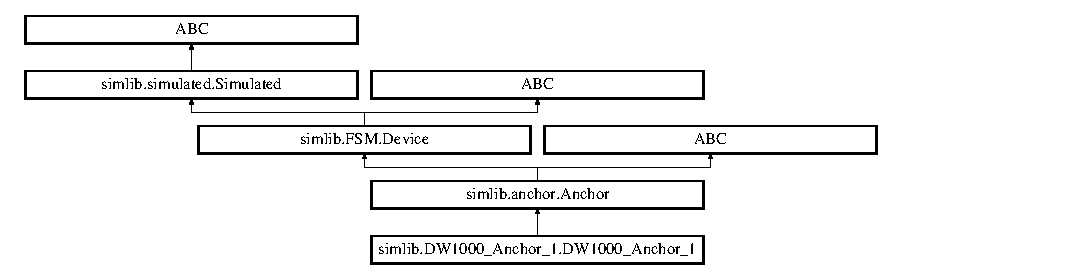
\includegraphics[height=4.000000cm]{classsimlib_1_1anchor_1_1_anchor}
\end{center}
\end{figure}
\subsection*{Public Member Functions}
\begin{DoxyCompactItemize}
\item 
def \mbox{\hyperlink{classsimlib_1_1anchor_1_1_anchor_a7f9c8d88a2b75c6906c7b3c407122253}{\+\_\+\+\_\+init\+\_\+\+\_\+}}
\item 
def \mbox{\hyperlink{classsimlib_1_1anchor_1_1_anchor_a07919385fe2be01caa5b21ecda72994a}{set\+Time}}
\item 
def \mbox{\hyperlink{classsimlib_1_1anchor_1_1_anchor_aad6e8cef879578483a4b76a82719b7bd}{get\+ID}} ()
\item 
def \mbox{\hyperlink{classsimlib_1_1anchor_1_1_anchor_a1bfd4394f56d62e710ed4df8367cb5a3}{listen\+For\+Signal}} ()
\item 
def \mbox{\hyperlink{classsimlib_1_1anchor_1_1_anchor_a99648f62d73c149e1683b829c3e3763c}{request\+Ping}}
\item 
def \mbox{\hyperlink{classsimlib_1_1anchor_1_1_anchor_a7fb5450523f88349670ecaee772996bc}{ping\+Node}}
\item 
def \mbox{\hyperlink{classsimlib_1_1anchor_1_1_anchor_ac9c49d6bb6cb2e736221dde820da32cd}{wait\+For\+Reply}}
\item 
def \mbox{\hyperlink{classsimlib_1_1anchor_1_1_anchor_a4766235728733695b9309020504d646e}{add\+Action}}
\item 
def \mbox{\hyperlink{classsimlib_1_1anchor_1_1_anchor_ad6a0662edca4f31fdb1f2e1ddc3f14f9}{prepend\+Action}}
\end{DoxyCompactItemize}
\subsection*{Public Attributes}
\begin{DoxyCompactItemize}
\item 
\mbox{\hyperlink{classsimlib_1_1anchor_1_1_anchor_a96058beb8928e45282047c32b54c91b0}{time}}
\item 
\mbox{\hyperlink{classsimlib_1_1anchor_1_1_anchor_a99d8dec757fbc70270e99c9c58c2af01}{ID}}
\item 
\mbox{\hyperlink{classsimlib_1_1anchor_1_1_anchor_a25728525e949903415a91e93835f25d1}{x\+Pos}}
\item 
\mbox{\hyperlink{classsimlib_1_1anchor_1_1_anchor_a8c2832ed33668293e7565ac92df91c09}{y\+Pos}}
\item 
\mbox{\hyperlink{classsimlib_1_1anchor_1_1_anchor_a9fe20f5528a2b23048ba1276fc20b916}{z\+Pos}}
\item 
\mbox{\hyperlink{classsimlib_1_1anchor_1_1_anchor_a0a3c5084cf1372dca4bf2e3e2929c70b}{pinged\+Node\+ID}}
\item 
\mbox{\hyperlink{classsimlib_1_1anchor_1_1_anchor_abba6bd8618826a157c3dc6449504b971}{measurement}}
\item 
\mbox{\hyperlink{classsimlib_1_1anchor_1_1_anchor_a455a6b6556f9daddf7ad9960b22378ab}{signal\+List}}
\item 
\mbox{\hyperlink{classsimlib_1_1anchor_1_1_anchor_a9ddf34bbd3d7e3ca151416b5d1bfea45}{distance}}
\end{DoxyCompactItemize}


\subsection{Constructor \& Destructor Documentation}
\mbox{\Hypertarget{classsimlib_1_1anchor_1_1_anchor_a7f9c8d88a2b75c6906c7b3c407122253}\label{classsimlib_1_1anchor_1_1_anchor_a7f9c8d88a2b75c6906c7b3c407122253}} 
\index{simlib\+::anchor\+::\+Anchor@{simlib\+::anchor\+::\+Anchor}!\+\_\+\+\_\+init\+\_\+\+\_\+@{\+\_\+\+\_\+init\+\_\+\+\_\+}}
\index{\+\_\+\+\_\+init\+\_\+\+\_\+@{\+\_\+\+\_\+init\+\_\+\+\_\+}!simlib\+::anchor\+::\+Anchor@{simlib\+::anchor\+::\+Anchor}}
\subsubsection{\texorpdfstring{\+\_\+\+\_\+init\+\_\+\+\_\+()}{\_\_init\_\_()}}
{\footnotesize\ttfamily def simlib.\+anchor.\+Anchor.\+\_\+\+\_\+init\+\_\+\+\_\+ (\begin{DoxyParamCaption}\item[{}]{self,  }\item[{}]{ID }\end{DoxyParamCaption})}



\subsection{Member Function Documentation}
\mbox{\Hypertarget{classsimlib_1_1anchor_1_1_anchor_a4766235728733695b9309020504d646e}\label{classsimlib_1_1anchor_1_1_anchor_a4766235728733695b9309020504d646e}} 
\index{simlib\+::anchor\+::\+Anchor@{simlib\+::anchor\+::\+Anchor}!add\+Action@{add\+Action}}
\index{add\+Action@{add\+Action}!simlib\+::anchor\+::\+Anchor@{simlib\+::anchor\+::\+Anchor}}
\subsubsection{\texorpdfstring{add\+Action()}{addAction()}}
{\footnotesize\ttfamily def simlib.\+anchor.\+Anchor.\+add\+Action (\begin{DoxyParamCaption}\item[{}]{self,  }\item[{}]{function }\end{DoxyParamCaption})}

\mbox{\Hypertarget{classsimlib_1_1anchor_1_1_anchor_aad6e8cef879578483a4b76a82719b7bd}\label{classsimlib_1_1anchor_1_1_anchor_aad6e8cef879578483a4b76a82719b7bd}} 
\index{simlib\+::anchor\+::\+Anchor@{simlib\+::anchor\+::\+Anchor}!get\+ID@{get\+ID}}
\index{get\+ID@{get\+ID}!simlib\+::anchor\+::\+Anchor@{simlib\+::anchor\+::\+Anchor}}
\subsubsection{\texorpdfstring{get\+I\+D()}{getID()}}
{\footnotesize\ttfamily def simlib.\+anchor.\+Anchor.\+get\+ID (\begin{DoxyParamCaption}\item[{}]{int }\end{DoxyParamCaption})}

\mbox{\Hypertarget{classsimlib_1_1anchor_1_1_anchor_a1bfd4394f56d62e710ed4df8367cb5a3}\label{classsimlib_1_1anchor_1_1_anchor_a1bfd4394f56d62e710ed4df8367cb5a3}} 
\index{simlib\+::anchor\+::\+Anchor@{simlib\+::anchor\+::\+Anchor}!listen\+For\+Signal@{listen\+For\+Signal}}
\index{listen\+For\+Signal@{listen\+For\+Signal}!simlib\+::anchor\+::\+Anchor@{simlib\+::anchor\+::\+Anchor}}
\subsubsection{\texorpdfstring{listen\+For\+Signal()}{listenForSignal()}}
{\footnotesize\ttfamily def simlib.\+anchor.\+Anchor.\+listen\+For\+Signal (\begin{DoxyParamCaption}\item[{}]{int }\end{DoxyParamCaption})}

\begin{DoxyVerb}Searches to see if it is the target of any signals. Returns the sending ID
if a signal is found or 0 if no signal is found.
\end{DoxyVerb}
 \mbox{\Hypertarget{classsimlib_1_1anchor_1_1_anchor_a7fb5450523f88349670ecaee772996bc}\label{classsimlib_1_1anchor_1_1_anchor_a7fb5450523f88349670ecaee772996bc}} 
\index{simlib\+::anchor\+::\+Anchor@{simlib\+::anchor\+::\+Anchor}!ping\+Node@{ping\+Node}}
\index{ping\+Node@{ping\+Node}!simlib\+::anchor\+::\+Anchor@{simlib\+::anchor\+::\+Anchor}}
\subsubsection{\texorpdfstring{ping\+Node()}{pingNode()}}
{\footnotesize\ttfamily def simlib.\+anchor.\+Anchor.\+ping\+Node (\begin{DoxyParamCaption}\item[{}]{self,  }\item[{}]{args }\end{DoxyParamCaption})}

\mbox{\Hypertarget{classsimlib_1_1anchor_1_1_anchor_ad6a0662edca4f31fdb1f2e1ddc3f14f9}\label{classsimlib_1_1anchor_1_1_anchor_ad6a0662edca4f31fdb1f2e1ddc3f14f9}} 
\index{simlib\+::anchor\+::\+Anchor@{simlib\+::anchor\+::\+Anchor}!prepend\+Action@{prepend\+Action}}
\index{prepend\+Action@{prepend\+Action}!simlib\+::anchor\+::\+Anchor@{simlib\+::anchor\+::\+Anchor}}
\subsubsection{\texorpdfstring{prepend\+Action()}{prependAction()}}
{\footnotesize\ttfamily def simlib.\+anchor.\+Anchor.\+prepend\+Action (\begin{DoxyParamCaption}\item[{}]{self,  }\item[{}]{function }\end{DoxyParamCaption})}

\mbox{\Hypertarget{classsimlib_1_1anchor_1_1_anchor_a99648f62d73c149e1683b829c3e3763c}\label{classsimlib_1_1anchor_1_1_anchor_a99648f62d73c149e1683b829c3e3763c}} 
\index{simlib\+::anchor\+::\+Anchor@{simlib\+::anchor\+::\+Anchor}!request\+Ping@{request\+Ping}}
\index{request\+Ping@{request\+Ping}!simlib\+::anchor\+::\+Anchor@{simlib\+::anchor\+::\+Anchor}}
\subsubsection{\texorpdfstring{request\+Ping()}{requestPing()}}
{\footnotesize\ttfamily def simlib.\+anchor.\+Anchor.\+request\+Ping (\begin{DoxyParamCaption}\item[{}]{self,  }\item[{}]{node }\end{DoxyParamCaption})}

\mbox{\Hypertarget{classsimlib_1_1anchor_1_1_anchor_a07919385fe2be01caa5b21ecda72994a}\label{classsimlib_1_1anchor_1_1_anchor_a07919385fe2be01caa5b21ecda72994a}} 
\index{simlib\+::anchor\+::\+Anchor@{simlib\+::anchor\+::\+Anchor}!set\+Time@{set\+Time}}
\index{set\+Time@{set\+Time}!simlib\+::anchor\+::\+Anchor@{simlib\+::anchor\+::\+Anchor}}
\subsubsection{\texorpdfstring{set\+Time()}{setTime()}}
{\footnotesize\ttfamily def simlib.\+anchor.\+Anchor.\+set\+Time (\begin{DoxyParamCaption}\item[{}]{time }\end{DoxyParamCaption})}

\mbox{\Hypertarget{classsimlib_1_1anchor_1_1_anchor_ac9c49d6bb6cb2e736221dde820da32cd}\label{classsimlib_1_1anchor_1_1_anchor_ac9c49d6bb6cb2e736221dde820da32cd}} 
\index{simlib\+::anchor\+::\+Anchor@{simlib\+::anchor\+::\+Anchor}!wait\+For\+Reply@{wait\+For\+Reply}}
\index{wait\+For\+Reply@{wait\+For\+Reply}!simlib\+::anchor\+::\+Anchor@{simlib\+::anchor\+::\+Anchor}}
\subsubsection{\texorpdfstring{wait\+For\+Reply()}{waitForReply()}}
{\footnotesize\ttfamily def simlib.\+anchor.\+Anchor.\+wait\+For\+Reply (\begin{DoxyParamCaption}\item[{}]{self,  }\item[{}]{args }\end{DoxyParamCaption})}



\subsection{Member Data Documentation}
\mbox{\Hypertarget{classsimlib_1_1anchor_1_1_anchor_a9ddf34bbd3d7e3ca151416b5d1bfea45}\label{classsimlib_1_1anchor_1_1_anchor_a9ddf34bbd3d7e3ca151416b5d1bfea45}} 
\index{simlib\+::anchor\+::\+Anchor@{simlib\+::anchor\+::\+Anchor}!distance@{distance}}
\index{distance@{distance}!simlib\+::anchor\+::\+Anchor@{simlib\+::anchor\+::\+Anchor}}
\subsubsection{\texorpdfstring{distance}{distance}}
{\footnotesize\ttfamily simlib.\+anchor.\+Anchor.\+distance}

\mbox{\Hypertarget{classsimlib_1_1anchor_1_1_anchor_a99d8dec757fbc70270e99c9c58c2af01}\label{classsimlib_1_1anchor_1_1_anchor_a99d8dec757fbc70270e99c9c58c2af01}} 
\index{simlib\+::anchor\+::\+Anchor@{simlib\+::anchor\+::\+Anchor}!ID@{ID}}
\index{ID@{ID}!simlib\+::anchor\+::\+Anchor@{simlib\+::anchor\+::\+Anchor}}
\subsubsection{\texorpdfstring{ID}{ID}}
{\footnotesize\ttfamily simlib.\+anchor.\+Anchor.\+ID}

\mbox{\Hypertarget{classsimlib_1_1anchor_1_1_anchor_abba6bd8618826a157c3dc6449504b971}\label{classsimlib_1_1anchor_1_1_anchor_abba6bd8618826a157c3dc6449504b971}} 
\index{simlib\+::anchor\+::\+Anchor@{simlib\+::anchor\+::\+Anchor}!measurement@{measurement}}
\index{measurement@{measurement}!simlib\+::anchor\+::\+Anchor@{simlib\+::anchor\+::\+Anchor}}
\subsubsection{\texorpdfstring{measurement}{measurement}}
{\footnotesize\ttfamily simlib.\+anchor.\+Anchor.\+measurement}

\mbox{\Hypertarget{classsimlib_1_1anchor_1_1_anchor_a0a3c5084cf1372dca4bf2e3e2929c70b}\label{classsimlib_1_1anchor_1_1_anchor_a0a3c5084cf1372dca4bf2e3e2929c70b}} 
\index{simlib\+::anchor\+::\+Anchor@{simlib\+::anchor\+::\+Anchor}!pinged\+Node\+ID@{pinged\+Node\+ID}}
\index{pinged\+Node\+ID@{pinged\+Node\+ID}!simlib\+::anchor\+::\+Anchor@{simlib\+::anchor\+::\+Anchor}}
\subsubsection{\texorpdfstring{pinged\+Node\+ID}{pingedNodeID}}
{\footnotesize\ttfamily simlib.\+anchor.\+Anchor.\+pinged\+Node\+ID}

\mbox{\Hypertarget{classsimlib_1_1anchor_1_1_anchor_a455a6b6556f9daddf7ad9960b22378ab}\label{classsimlib_1_1anchor_1_1_anchor_a455a6b6556f9daddf7ad9960b22378ab}} 
\index{simlib\+::anchor\+::\+Anchor@{simlib\+::anchor\+::\+Anchor}!signal\+List@{signal\+List}}
\index{signal\+List@{signal\+List}!simlib\+::anchor\+::\+Anchor@{simlib\+::anchor\+::\+Anchor}}
\subsubsection{\texorpdfstring{signal\+List}{signalList}}
{\footnotesize\ttfamily simlib.\+anchor.\+Anchor.\+signal\+List}

\mbox{\Hypertarget{classsimlib_1_1anchor_1_1_anchor_a96058beb8928e45282047c32b54c91b0}\label{classsimlib_1_1anchor_1_1_anchor_a96058beb8928e45282047c32b54c91b0}} 
\index{simlib\+::anchor\+::\+Anchor@{simlib\+::anchor\+::\+Anchor}!time@{time}}
\index{time@{time}!simlib\+::anchor\+::\+Anchor@{simlib\+::anchor\+::\+Anchor}}
\subsubsection{\texorpdfstring{time}{time}}
{\footnotesize\ttfamily simlib.\+anchor.\+Anchor.\+time}

\mbox{\Hypertarget{classsimlib_1_1anchor_1_1_anchor_a25728525e949903415a91e93835f25d1}\label{classsimlib_1_1anchor_1_1_anchor_a25728525e949903415a91e93835f25d1}} 
\index{simlib\+::anchor\+::\+Anchor@{simlib\+::anchor\+::\+Anchor}!x\+Pos@{x\+Pos}}
\index{x\+Pos@{x\+Pos}!simlib\+::anchor\+::\+Anchor@{simlib\+::anchor\+::\+Anchor}}
\subsubsection{\texorpdfstring{x\+Pos}{xPos}}
{\footnotesize\ttfamily simlib.\+anchor.\+Anchor.\+x\+Pos}

\mbox{\Hypertarget{classsimlib_1_1anchor_1_1_anchor_a8c2832ed33668293e7565ac92df91c09}\label{classsimlib_1_1anchor_1_1_anchor_a8c2832ed33668293e7565ac92df91c09}} 
\index{simlib\+::anchor\+::\+Anchor@{simlib\+::anchor\+::\+Anchor}!y\+Pos@{y\+Pos}}
\index{y\+Pos@{y\+Pos}!simlib\+::anchor\+::\+Anchor@{simlib\+::anchor\+::\+Anchor}}
\subsubsection{\texorpdfstring{y\+Pos}{yPos}}
{\footnotesize\ttfamily simlib.\+anchor.\+Anchor.\+y\+Pos}

\mbox{\Hypertarget{classsimlib_1_1anchor_1_1_anchor_a9fe20f5528a2b23048ba1276fc20b916}\label{classsimlib_1_1anchor_1_1_anchor_a9fe20f5528a2b23048ba1276fc20b916}} 
\index{simlib\+::anchor\+::\+Anchor@{simlib\+::anchor\+::\+Anchor}!z\+Pos@{z\+Pos}}
\index{z\+Pos@{z\+Pos}!simlib\+::anchor\+::\+Anchor@{simlib\+::anchor\+::\+Anchor}}
\subsubsection{\texorpdfstring{z\+Pos}{zPos}}
{\footnotesize\ttfamily simlib.\+anchor.\+Anchor.\+z\+Pos}



The documentation for this class was generated from the following file\+:\begin{DoxyCompactItemize}
\item 
\mbox{\hyperlink{anchor_8py}{anchor.\+py}}\end{DoxyCompactItemize}

\hypertarget{classsimlib_1_1archspec_1_1_arch_spec}{}\section{simlib.\+archspec.\+Arch\+Spec Class Reference}
\label{classsimlib_1_1archspec_1_1_arch_spec}\index{simlib.\+archspec.\+Arch\+Spec@{simlib.\+archspec.\+Arch\+Spec}}


Classes \#\#.  


\subsection*{Public Member Functions}
\begin{DoxyCompactItemize}
\item 
def \mbox{\hyperlink{classsimlib_1_1archspec_1_1_arch_spec_a6632a5eed5f33524fa2a6a51a4f01274}{\+\_\+\+\_\+init\+\_\+\+\_\+}}
\item 
def \mbox{\hyperlink{classsimlib_1_1archspec_1_1_arch_spec_a630555d33bafc4fda4e3ef4a4a856b13}{get\+\_\+hubclass}} (self)
\item 
def \mbox{\hyperlink{classsimlib_1_1archspec_1_1_arch_spec_aca0be1948149b2a220106d5bb4bc3c56}{get\+\_\+anchorclass}} (self)
\item 
def \mbox{\hyperlink{classsimlib_1_1archspec_1_1_arch_spec_a731ef67f540e5961937ccda28babfe21}{get\+\_\+nodeclass}} (self)
\item 
def \mbox{\hyperlink{classsimlib_1_1archspec_1_1_arch_spec_a5419a0d3b27b4864a9cea18f3f42ec2f}{set\+\_\+hubclass}}
\item 
def \mbox{\hyperlink{classsimlib_1_1archspec_1_1_arch_spec_afb99f1d749346f5336ecdd6ff9d1cce6}{set\+\_\+anchorclass}}
\item 
def \mbox{\hyperlink{classsimlib_1_1archspec_1_1_arch_spec_a083a2500010362bcd18101dcf1cc6e6d}{set\+\_\+nodeclass}}
\end{DoxyCompactItemize}


\subsection{Detailed Description}
Classes \#\#. 

\begin{DoxyVerb}Architecture specification
Defines what classes to use for hub, anchors, and nodes.
\end{DoxyVerb}
 \begin{DoxyVerb}The default constructor
@param hubclass The type of the central hub
@param anchorclass The type of the anchor
@param nodeclass The type of the node
\end{DoxyVerb}
 

\subsection{Constructor \& Destructor Documentation}
\mbox{\Hypertarget{classsimlib_1_1archspec_1_1_arch_spec_a6632a5eed5f33524fa2a6a51a4f01274}\label{classsimlib_1_1archspec_1_1_arch_spec_a6632a5eed5f33524fa2a6a51a4f01274}} 
\index{simlib\+::archspec\+::\+Arch\+Spec@{simlib\+::archspec\+::\+Arch\+Spec}!\+\_\+\+\_\+init\+\_\+\+\_\+@{\+\_\+\+\_\+init\+\_\+\+\_\+}}
\index{\+\_\+\+\_\+init\+\_\+\+\_\+@{\+\_\+\+\_\+init\+\_\+\+\_\+}!simlib\+::archspec\+::\+Arch\+Spec@{simlib\+::archspec\+::\+Arch\+Spec}}
\subsubsection{\texorpdfstring{\+\_\+\+\_\+init\+\_\+\+\_\+()}{\_\_init\_\_()}}
{\footnotesize\ttfamily def simlib.\+archspec.\+Arch\+Spec.\+\_\+\+\_\+init\+\_\+\+\_\+ (\begin{DoxyParamCaption}\item[{}]{self,  }\item[{}]{hubclass }\end{DoxyParamCaption})}



\subsection{Member Function Documentation}
\mbox{\Hypertarget{classsimlib_1_1archspec_1_1_arch_spec_aca0be1948149b2a220106d5bb4bc3c56}\label{classsimlib_1_1archspec_1_1_arch_spec_aca0be1948149b2a220106d5bb4bc3c56}} 
\index{simlib\+::archspec\+::\+Arch\+Spec@{simlib\+::archspec\+::\+Arch\+Spec}!get\+\_\+anchorclass@{get\+\_\+anchorclass}}
\index{get\+\_\+anchorclass@{get\+\_\+anchorclass}!simlib\+::archspec\+::\+Arch\+Spec@{simlib\+::archspec\+::\+Arch\+Spec}}
\subsubsection{\texorpdfstring{get\+\_\+anchorclass()}{get\_anchorclass()}}
{\footnotesize\ttfamily def simlib.\+archspec.\+Arch\+Spec.\+get\+\_\+anchorclass (\begin{DoxyParamCaption}\item[{}]{self,  }\item[{}]{type }\end{DoxyParamCaption})}

\mbox{\Hypertarget{classsimlib_1_1archspec_1_1_arch_spec_a630555d33bafc4fda4e3ef4a4a856b13}\label{classsimlib_1_1archspec_1_1_arch_spec_a630555d33bafc4fda4e3ef4a4a856b13}} 
\index{simlib\+::archspec\+::\+Arch\+Spec@{simlib\+::archspec\+::\+Arch\+Spec}!get\+\_\+hubclass@{get\+\_\+hubclass}}
\index{get\+\_\+hubclass@{get\+\_\+hubclass}!simlib\+::archspec\+::\+Arch\+Spec@{simlib\+::archspec\+::\+Arch\+Spec}}
\subsubsection{\texorpdfstring{get\+\_\+hubclass()}{get\_hubclass()}}
{\footnotesize\ttfamily def simlib.\+archspec.\+Arch\+Spec.\+get\+\_\+hubclass (\begin{DoxyParamCaption}\item[{}]{self,  }\item[{}]{type }\end{DoxyParamCaption})}

\mbox{\Hypertarget{classsimlib_1_1archspec_1_1_arch_spec_a731ef67f540e5961937ccda28babfe21}\label{classsimlib_1_1archspec_1_1_arch_spec_a731ef67f540e5961937ccda28babfe21}} 
\index{simlib\+::archspec\+::\+Arch\+Spec@{simlib\+::archspec\+::\+Arch\+Spec}!get\+\_\+nodeclass@{get\+\_\+nodeclass}}
\index{get\+\_\+nodeclass@{get\+\_\+nodeclass}!simlib\+::archspec\+::\+Arch\+Spec@{simlib\+::archspec\+::\+Arch\+Spec}}
\subsubsection{\texorpdfstring{get\+\_\+nodeclass()}{get\_nodeclass()}}
{\footnotesize\ttfamily def simlib.\+archspec.\+Arch\+Spec.\+get\+\_\+nodeclass (\begin{DoxyParamCaption}\item[{}]{self,  }\item[{}]{type }\end{DoxyParamCaption})}

\mbox{\Hypertarget{classsimlib_1_1archspec_1_1_arch_spec_afb99f1d749346f5336ecdd6ff9d1cce6}\label{classsimlib_1_1archspec_1_1_arch_spec_afb99f1d749346f5336ecdd6ff9d1cce6}} 
\index{simlib\+::archspec\+::\+Arch\+Spec@{simlib\+::archspec\+::\+Arch\+Spec}!set\+\_\+anchorclass@{set\+\_\+anchorclass}}
\index{set\+\_\+anchorclass@{set\+\_\+anchorclass}!simlib\+::archspec\+::\+Arch\+Spec@{simlib\+::archspec\+::\+Arch\+Spec}}
\subsubsection{\texorpdfstring{set\+\_\+anchorclass()}{set\_anchorclass()}}
{\footnotesize\ttfamily def simlib.\+archspec.\+Arch\+Spec.\+set\+\_\+anchorclass (\begin{DoxyParamCaption}\item[{}]{self,  }\item[{}]{anchorclass }\end{DoxyParamCaption})}

\mbox{\Hypertarget{classsimlib_1_1archspec_1_1_arch_spec_a5419a0d3b27b4864a9cea18f3f42ec2f}\label{classsimlib_1_1archspec_1_1_arch_spec_a5419a0d3b27b4864a9cea18f3f42ec2f}} 
\index{simlib\+::archspec\+::\+Arch\+Spec@{simlib\+::archspec\+::\+Arch\+Spec}!set\+\_\+hubclass@{set\+\_\+hubclass}}
\index{set\+\_\+hubclass@{set\+\_\+hubclass}!simlib\+::archspec\+::\+Arch\+Spec@{simlib\+::archspec\+::\+Arch\+Spec}}
\subsubsection{\texorpdfstring{set\+\_\+hubclass()}{set\_hubclass()}}
{\footnotesize\ttfamily def simlib.\+archspec.\+Arch\+Spec.\+set\+\_\+hubclass (\begin{DoxyParamCaption}\item[{}]{self,  }\item[{}]{hubclass }\end{DoxyParamCaption})}

\mbox{\Hypertarget{classsimlib_1_1archspec_1_1_arch_spec_a083a2500010362bcd18101dcf1cc6e6d}\label{classsimlib_1_1archspec_1_1_arch_spec_a083a2500010362bcd18101dcf1cc6e6d}} 
\index{simlib\+::archspec\+::\+Arch\+Spec@{simlib\+::archspec\+::\+Arch\+Spec}!set\+\_\+nodeclass@{set\+\_\+nodeclass}}
\index{set\+\_\+nodeclass@{set\+\_\+nodeclass}!simlib\+::archspec\+::\+Arch\+Spec@{simlib\+::archspec\+::\+Arch\+Spec}}
\subsubsection{\texorpdfstring{set\+\_\+nodeclass()}{set\_nodeclass()}}
{\footnotesize\ttfamily def simlib.\+archspec.\+Arch\+Spec.\+set\+\_\+nodeclass (\begin{DoxyParamCaption}\item[{}]{self,  }\item[{}]{nodeclass }\end{DoxyParamCaption})}



The documentation for this class was generated from the following file\+:\begin{DoxyCompactItemize}
\item 
\mbox{\hyperlink{archspec_8py}{archspec.\+py}}\end{DoxyCompactItemize}

\hypertarget{classsimlib_1_1_f_s_m_1_1_device}{}\section{simlib.\+F\+S\+M.\+Device Class Reference}
\label{classsimlib_1_1_f_s_m_1_1_device}\index{simlib.\+F\+S\+M.\+Device@{simlib.\+F\+S\+M.\+Device}}
Inheritance diagram for simlib.\+F\+S\+M.\+Device\+:\begin{figure}[H]
\begin{center}
\leavevmode
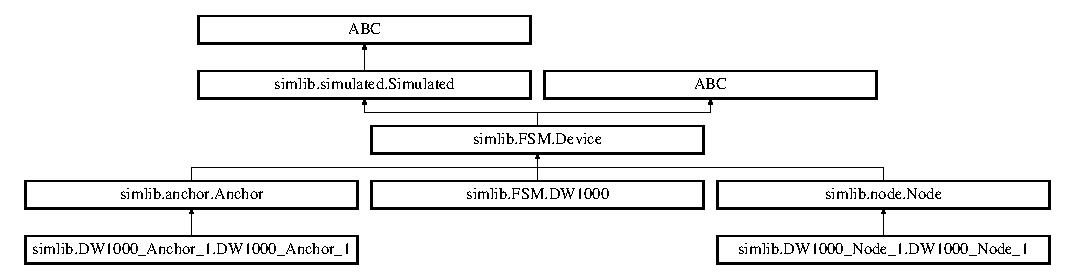
\includegraphics[height=3.321471cm]{classsimlib_1_1_f_s_m_1_1_device}
\end{center}
\end{figure}
\subsection*{Public Member Functions}
\begin{DoxyCompactItemize}
\item 
\mbox{\Hypertarget{classsimlib_1_1_f_s_m_1_1_device_a5696250d05d766c549c37faa84db7693}\label{classsimlib_1_1_f_s_m_1_1_device_a5696250d05d766c549c37faa84db7693}} 
def {\bfseries \+\_\+\+\_\+init\+\_\+\+\_\+} (self)
\item 
\mbox{\Hypertarget{classsimlib_1_1_f_s_m_1_1_device_a306e757fa92528b888de0f1b00b0be5c}\label{classsimlib_1_1_f_s_m_1_1_device_a306e757fa92528b888de0f1b00b0be5c}} 
def {\bfseries \+\_\+\+\_\+init\+\_\+\+\_\+}
\item 
def \mbox{\hyperlink{classsimlib_1_1_f_s_m_1_1_device_a2f0fc2dd8e6da5688c00ed2004538abb}{get\+State}} (self)
\item 
def \mbox{\hyperlink{classsimlib_1_1_f_s_m_1_1_device_a66671fefc8ed8e04091244d40ae9eb41}{get\+Available\+Next\+States}} (self)
\item 
\mbox{\Hypertarget{classsimlib_1_1_f_s_m_1_1_device_a816c8a7e8c01c9d8e7748f083903466a}\label{classsimlib_1_1_f_s_m_1_1_device_a816c8a7e8c01c9d8e7748f083903466a}} 
def {\bfseries set\+Next\+State}
\item 
\mbox{\Hypertarget{classsimlib_1_1_f_s_m_1_1_device_a82fec7b5aa14a400069f9170640c8666}\label{classsimlib_1_1_f_s_m_1_1_device_a82fec7b5aa14a400069f9170640c8666}} 
def {\bfseries get\+Param}
\end{DoxyCompactItemize}
\subsection*{Public Attributes}
\begin{DoxyCompactItemize}
\item 
\mbox{\Hypertarget{classsimlib_1_1_f_s_m_1_1_device_af6a460115a317bf2705479cc12ebcb81}\label{classsimlib_1_1_f_s_m_1_1_device_af6a460115a317bf2705479cc12ebcb81}} 
{\bfseries available\+\_\+states}
\item 
\mbox{\Hypertarget{classsimlib_1_1_f_s_m_1_1_device_aa931047c9f7d959f59e23e968e70d2c6}\label{classsimlib_1_1_f_s_m_1_1_device_aa931047c9f7d959f59e23e968e70d2c6}} 
{\bfseries initial\+\_\+state}
\item 
\mbox{\Hypertarget{classsimlib_1_1_f_s_m_1_1_device_ac59c9ebe10d83f78f0840f5e1eb6d351}\label{classsimlib_1_1_f_s_m_1_1_device_ac59c9ebe10d83f78f0840f5e1eb6d351}} 
{\bfseries dev\+\_\+state}
\item 
\mbox{\Hypertarget{classsimlib_1_1_f_s_m_1_1_device_a3fc1af3d8a1500d7b27e4ad6a80dca59}\label{classsimlib_1_1_f_s_m_1_1_device_a3fc1af3d8a1500d7b27e4ad6a80dca59}} 
{\bfseries physical\+\_\+data}
\item 
\mbox{\Hypertarget{classsimlib_1_1_f_s_m_1_1_device_a90f519879573a37f7200618a70b02218}\label{classsimlib_1_1_f_s_m_1_1_device_a90f519879573a37f7200618a70b02218}} 
{\bfseries next\+\_\+states}
\end{DoxyCompactItemize}


\subsection{Detailed Description}
\begin{DoxyVerb}Creates an instance of a device dependent on the FSM,
physical data, and available states used to accurately
model the DW1000 or other like devices. 
\end{DoxyVerb}
 

\subsection{Member Function Documentation}
\mbox{\Hypertarget{classsimlib_1_1_f_s_m_1_1_device_a66671fefc8ed8e04091244d40ae9eb41}\label{classsimlib_1_1_f_s_m_1_1_device_a66671fefc8ed8e04091244d40ae9eb41}} 
\index{simlib\+::\+F\+S\+M\+::\+Device@{simlib\+::\+F\+S\+M\+::\+Device}!get\+Available\+Next\+States@{get\+Available\+Next\+States}}
\index{get\+Available\+Next\+States@{get\+Available\+Next\+States}!simlib\+::\+F\+S\+M\+::\+Device@{simlib\+::\+F\+S\+M\+::\+Device}}
\subsubsection{\texorpdfstring{get\+Available\+Next\+States()}{getAvailableNextStates()}}
{\footnotesize\ttfamily def simlib.\+F\+S\+M.\+Device.\+get\+Available\+Next\+States (\begin{DoxyParamCaption}\item[{}]{self }\end{DoxyParamCaption})}

\begin{DoxyVerb}Gets the possible next states from the FSM
and assigns them to the next_states.
\end{DoxyVerb}
 \mbox{\Hypertarget{classsimlib_1_1_f_s_m_1_1_device_a2f0fc2dd8e6da5688c00ed2004538abb}\label{classsimlib_1_1_f_s_m_1_1_device_a2f0fc2dd8e6da5688c00ed2004538abb}} 
\index{simlib\+::\+F\+S\+M\+::\+Device@{simlib\+::\+F\+S\+M\+::\+Device}!get\+State@{get\+State}}
\index{get\+State@{get\+State}!simlib\+::\+F\+S\+M\+::\+Device@{simlib\+::\+F\+S\+M\+::\+Device}}
\subsubsection{\texorpdfstring{get\+State()}{getState()}}
{\footnotesize\ttfamily def simlib.\+F\+S\+M.\+Device.\+get\+State (\begin{DoxyParamCaption}\item[{}]{self,  }\item[{}]{State }\end{DoxyParamCaption})}

\begin{DoxyVerb}Returns the current state of the device. 
\end{DoxyVerb}
 

The documentation for this class was generated from the following file\+:\begin{DoxyCompactItemize}
\item 
src/simlib/F\+S\+M.\+py\end{DoxyCompactItemize}

\hypertarget{classsimlib_1_1_f_s_m_1_1_d_w1000}{}\section{simlib.\+F\+S\+M.\+D\+W1000 Class Reference}
\label{classsimlib_1_1_f_s_m_1_1_d_w1000}\index{simlib.\+F\+S\+M.\+D\+W1000@{simlib.\+F\+S\+M.\+D\+W1000}}
Inheritance diagram for simlib.\+F\+S\+M.\+D\+W1000\+:\begin{figure}[H]
\begin{center}
\leavevmode
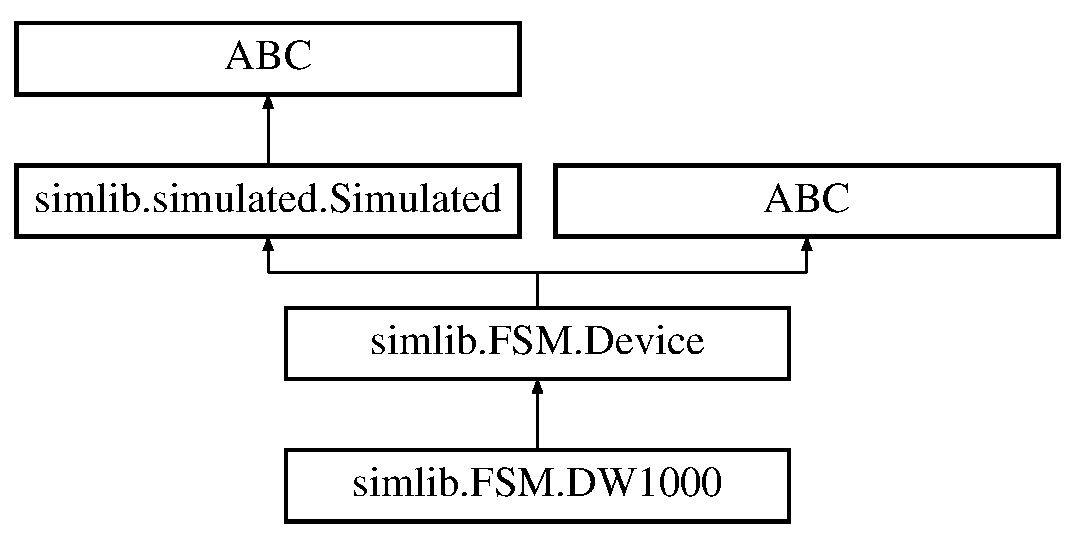
\includegraphics[height=4.000000cm]{classsimlib_1_1_f_s_m_1_1_d_w1000}
\end{center}
\end{figure}
\subsection*{Public Member Functions}
\begin{DoxyCompactItemize}
\item 
def \mbox{\hyperlink{classsimlib_1_1_f_s_m_1_1_d_w1000_a0c91896ce1517bade299a3a905b3c26c}{\+\_\+\+\_\+init\+\_\+\+\_\+}}
\item 
def \mbox{\hyperlink{classsimlib_1_1_f_s_m_1_1_d_w1000_aa91a241f59daa1f2479f0d19f60c6124}{mainloop}}
\end{DoxyCompactItemize}
\subsection*{Additional Inherited Members}


\subsection{Constructor \& Destructor Documentation}
\mbox{\Hypertarget{classsimlib_1_1_f_s_m_1_1_d_w1000_a0c91896ce1517bade299a3a905b3c26c}\label{classsimlib_1_1_f_s_m_1_1_d_w1000_a0c91896ce1517bade299a3a905b3c26c}} 
\index{simlib\+::\+F\+S\+M\+::\+D\+W1000@{simlib\+::\+F\+S\+M\+::\+D\+W1000}!\+\_\+\+\_\+init\+\_\+\+\_\+@{\+\_\+\+\_\+init\+\_\+\+\_\+}}
\index{\+\_\+\+\_\+init\+\_\+\+\_\+@{\+\_\+\+\_\+init\+\_\+\+\_\+}!simlib\+::\+F\+S\+M\+::\+D\+W1000@{simlib\+::\+F\+S\+M\+::\+D\+W1000}}
\subsubsection{\texorpdfstring{\+\_\+\+\_\+init\+\_\+\+\_\+()}{\_\_init\_\_()}}
{\footnotesize\ttfamily def simlib.\+F\+S\+M.\+D\+W1000.\+\_\+\+\_\+init\+\_\+\+\_\+ (\begin{DoxyParamCaption}\item[{}]{self,  }\item[{}]{available\+\_\+states }\end{DoxyParamCaption})}



\subsection{Member Function Documentation}
\mbox{\Hypertarget{classsimlib_1_1_f_s_m_1_1_d_w1000_aa91a241f59daa1f2479f0d19f60c6124}\label{classsimlib_1_1_f_s_m_1_1_d_w1000_aa91a241f59daa1f2479f0d19f60c6124}} 
\index{simlib\+::\+F\+S\+M\+::\+D\+W1000@{simlib\+::\+F\+S\+M\+::\+D\+W1000}!mainloop@{mainloop}}
\index{mainloop@{mainloop}!simlib\+::\+F\+S\+M\+::\+D\+W1000@{simlib\+::\+F\+S\+M\+::\+D\+W1000}}
\subsubsection{\texorpdfstring{mainloop()}{mainloop()}}
{\footnotesize\ttfamily def simlib.\+F\+S\+M.\+D\+W1000.\+mainloop (\begin{DoxyParamCaption}\item[{}]{self,  }\item[{}]{simlist }\end{DoxyParamCaption})}



The documentation for this class was generated from the following file\+:\begin{DoxyCompactItemize}
\item 
\mbox{\hyperlink{_f_s_m_8py}{F\+S\+M.\+py}}\end{DoxyCompactItemize}

\hypertarget{classsimlib_1_1_d_w1000___anchor__1_1_1_d_w1000___anchor__1}{}\section{simlib.\+D\+W1000\+\_\+\+Anchor\+\_\+1.\+D\+W1000\+\_\+\+Anchor\+\_\+1 Class Reference}
\label{classsimlib_1_1_d_w1000___anchor__1_1_1_d_w1000___anchor__1}\index{simlib.\+D\+W1000\+\_\+\+Anchor\+\_\+1.\+D\+W1000\+\_\+\+Anchor\+\_\+1@{simlib.\+D\+W1000\+\_\+\+Anchor\+\_\+1.\+D\+W1000\+\_\+\+Anchor\+\_\+1}}
Inheritance diagram for simlib.\+D\+W1000\+\_\+\+Anchor\+\_\+1.\+D\+W1000\+\_\+\+Anchor\+\_\+1\+:\begin{figure}[H]
\begin{center}
\leavevmode
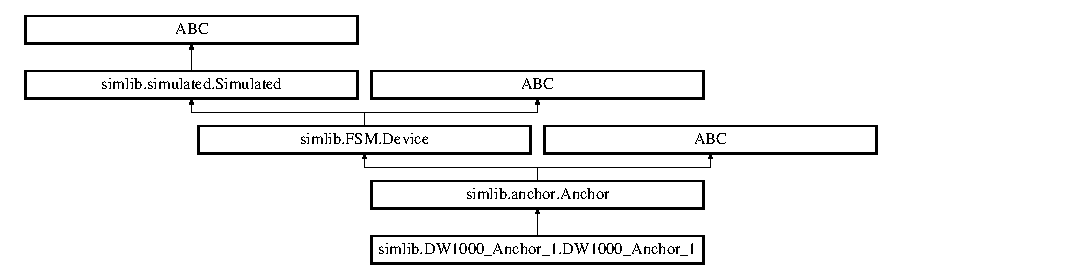
\includegraphics[height=3.321471cm]{classsimlib_1_1_d_w1000___anchor__1_1_1_d_w1000___anchor__1}
\end{center}
\end{figure}
\subsection*{Public Member Functions}
\begin{DoxyCompactItemize}
\item 
\mbox{\Hypertarget{classsimlib_1_1_d_w1000___anchor__1_1_1_d_w1000___anchor__1_aa085714e3ff120a3e501b21a2f247932}\label{classsimlib_1_1_d_w1000___anchor__1_1_1_d_w1000___anchor__1_aa085714e3ff120a3e501b21a2f247932}} 
def {\bfseries \+\_\+\+\_\+init\+\_\+\+\_\+}
\item 
\mbox{\Hypertarget{classsimlib_1_1_d_w1000___anchor__1_1_1_d_w1000___anchor__1_aba6174e81ab331e03f8181d5cb22b15a}\label{classsimlib_1_1_d_w1000___anchor__1_1_1_d_w1000___anchor__1_aba6174e81ab331e03f8181d5cb22b15a}} 
def {\bfseries get\+Off\+Current} (physical\+\_\+data)
\item 
\mbox{\Hypertarget{classsimlib_1_1_d_w1000___anchor__1_1_1_d_w1000___anchor__1_a34d5bb222767b035aee255a5afce53da}\label{classsimlib_1_1_d_w1000___anchor__1_1_1_d_w1000___anchor__1_a34d5bb222767b035aee255a5afce53da}} 
def {\bfseries get\+Deep\+Sleep\+Current} (physical\+\_\+data)
\item 
\mbox{\Hypertarget{classsimlib_1_1_d_w1000___anchor__1_1_1_d_w1000___anchor__1_a7fe142641babd9b567d85b9cd89526b6}\label{classsimlib_1_1_d_w1000___anchor__1_1_1_d_w1000___anchor__1_a7fe142641babd9b567d85b9cd89526b6}} 
def {\bfseries get\+Sleep\+Current} (physical\+\_\+data)
\item 
\mbox{\Hypertarget{classsimlib_1_1_d_w1000___anchor__1_1_1_d_w1000___anchor__1_a14f23ace38a77c3c9dc7db13b3db0630}\label{classsimlib_1_1_d_w1000___anchor__1_1_1_d_w1000___anchor__1_a14f23ace38a77c3c9dc7db13b3db0630}} 
def {\bfseries get\+Init\+Current} (physical\+\_\+data)
\item 
\mbox{\Hypertarget{classsimlib_1_1_d_w1000___anchor__1_1_1_d_w1000___anchor__1_a90ec565857e0e6d07936f128dbc664d4}\label{classsimlib_1_1_d_w1000___anchor__1_1_1_d_w1000___anchor__1_a90ec565857e0e6d07936f128dbc664d4}} 
def {\bfseries get\+Idle\+Current} (physical\+\_\+data)
\item 
\mbox{\Hypertarget{classsimlib_1_1_d_w1000___anchor__1_1_1_d_w1000___anchor__1_a5328108cb2ec8ca81f8c73496ee9afc0}\label{classsimlib_1_1_d_w1000___anchor__1_1_1_d_w1000___anchor__1_a5328108cb2ec8ca81f8c73496ee9afc0}} 
def {\bfseries get\+R\+X\+Current} (physical\+\_\+data)
\item 
\mbox{\Hypertarget{classsimlib_1_1_d_w1000___anchor__1_1_1_d_w1000___anchor__1_a64ae3243971710997d2ae172de12b404}\label{classsimlib_1_1_d_w1000___anchor__1_1_1_d_w1000___anchor__1_a64ae3243971710997d2ae172de12b404}} 
def {\bfseries get\+T\+X\+Current} (physical\+\_\+data)
\item 
\mbox{\Hypertarget{classsimlib_1_1_d_w1000___anchor__1_1_1_d_w1000___anchor__1_a46b306f8af2e3ac1e71ab32540f1bdd0}\label{classsimlib_1_1_d_w1000___anchor__1_1_1_d_w1000___anchor__1_a46b306f8af2e3ac1e71ab32540f1bdd0}} 
def {\bfseries get\+Time} (physical\+\_\+data)
\item 
\mbox{\Hypertarget{classsimlib_1_1_d_w1000___anchor__1_1_1_d_w1000___anchor__1_ad334ae70db4ceca36f290658894d7134}\label{classsimlib_1_1_d_w1000___anchor__1_1_1_d_w1000___anchor__1_ad334ae70db4ceca36f290658894d7134}} 
def {\bfseries get\+Battery} (dev\+\_\+data, state\+\_\+data)
\item 
\mbox{\Hypertarget{classsimlib_1_1_d_w1000___anchor__1_1_1_d_w1000___anchor__1_ae73367697bcd7001baf76f0583f8e295}\label{classsimlib_1_1_d_w1000___anchor__1_1_1_d_w1000___anchor__1_ae73367697bcd7001baf76f0583f8e295}} 
def {\bfseries mainloop} (self)
\end{DoxyCompactItemize}
\subsection*{Public Attributes}
\begin{DoxyCompactItemize}
\item 
\mbox{\Hypertarget{classsimlib_1_1_d_w1000___anchor__1_1_1_d_w1000___anchor__1_ad98bffdd8c03847d372727edcf19d59d}\label{classsimlib_1_1_d_w1000___anchor__1_1_1_d_w1000___anchor__1_ad98bffdd8c03847d372727edcf19d59d}} 
{\bfseries available\+\_\+states}
\item 
\mbox{\Hypertarget{classsimlib_1_1_d_w1000___anchor__1_1_1_d_w1000___anchor__1_a98f1c19fbde45956f3a1e09b2cd9d89a}\label{classsimlib_1_1_d_w1000___anchor__1_1_1_d_w1000___anchor__1_a98f1c19fbde45956f3a1e09b2cd9d89a}} 
{\bfseries initial\+\_\+state}
\item 
\mbox{\Hypertarget{classsimlib_1_1_d_w1000___anchor__1_1_1_d_w1000___anchor__1_ace5c57689a3b5ed4f5d404d9ef0660ab}\label{classsimlib_1_1_d_w1000___anchor__1_1_1_d_w1000___anchor__1_ace5c57689a3b5ed4f5d404d9ef0660ab}} 
{\bfseries dev\+\_\+state}
\item 
\mbox{\Hypertarget{classsimlib_1_1_d_w1000___anchor__1_1_1_d_w1000___anchor__1_aadcde7bf26965a132040961a7ddfc627}\label{classsimlib_1_1_d_w1000___anchor__1_1_1_d_w1000___anchor__1_aadcde7bf26965a132040961a7ddfc627}} 
{\bfseries physical\+\_\+data}
\item 
\mbox{\Hypertarget{classsimlib_1_1_d_w1000___anchor__1_1_1_d_w1000___anchor__1_a852645997e25e304378d4d80442bda41}\label{classsimlib_1_1_d_w1000___anchor__1_1_1_d_w1000___anchor__1_a852645997e25e304378d4d80442bda41}} 
{\bfseries next\+\_\+states}
\end{DoxyCompactItemize}


The documentation for this class was generated from the following file\+:\begin{DoxyCompactItemize}
\item 
src/simlib/D\+W1000\+\_\+\+Anchor\+\_\+1.\+py\end{DoxyCompactItemize}

\hypertarget{classsimlib_1_1_d_w1000___node__1_1_1_d_w1000___node__1}{}\section{simlib.\+D\+W1000\+\_\+\+Node\+\_\+1.\+D\+W1000\+\_\+\+Node\+\_\+1 Class Reference}
\label{classsimlib_1_1_d_w1000___node__1_1_1_d_w1000___node__1}\index{simlib.\+D\+W1000\+\_\+\+Node\+\_\+1.\+D\+W1000\+\_\+\+Node\+\_\+1@{simlib.\+D\+W1000\+\_\+\+Node\+\_\+1.\+D\+W1000\+\_\+\+Node\+\_\+1}}
Inheritance diagram for simlib.\+D\+W1000\+\_\+\+Node\+\_\+1.\+D\+W1000\+\_\+\+Node\+\_\+1\+:\begin{figure}[H]
\begin{center}
\leavevmode
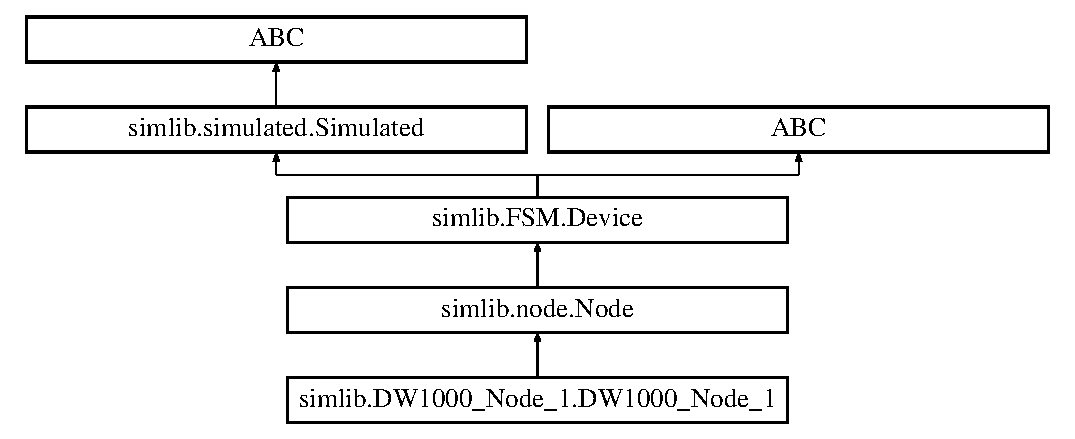
\includegraphics[height=5.000000cm]{classsimlib_1_1_d_w1000___node__1_1_1_d_w1000___node__1}
\end{center}
\end{figure}
\subsection*{Public Member Functions}
\begin{DoxyCompactItemize}
\item 
\mbox{\Hypertarget{classsimlib_1_1_d_w1000___node__1_1_1_d_w1000___node__1_a8c341481ea3215ac5296b6ad06bf4012}\label{classsimlib_1_1_d_w1000___node__1_1_1_d_w1000___node__1_a8c341481ea3215ac5296b6ad06bf4012}} 
def {\bfseries \+\_\+\+\_\+init\+\_\+\+\_\+}
\item 
\mbox{\Hypertarget{classsimlib_1_1_d_w1000___node__1_1_1_d_w1000___node__1_ab1a05766285beaa124d1ed3bfbf7d7cc}\label{classsimlib_1_1_d_w1000___node__1_1_1_d_w1000___node__1_ab1a05766285beaa124d1ed3bfbf7d7cc}} 
def {\bfseries get\+Off\+Current} (physical\+\_\+data)
\item 
\mbox{\Hypertarget{classsimlib_1_1_d_w1000___node__1_1_1_d_w1000___node__1_a6ebd74794cbbc8884ea9882c15949ae0}\label{classsimlib_1_1_d_w1000___node__1_1_1_d_w1000___node__1_a6ebd74794cbbc8884ea9882c15949ae0}} 
def {\bfseries get\+Deep\+Sleep\+Current} (physical\+\_\+data)
\item 
\mbox{\Hypertarget{classsimlib_1_1_d_w1000___node__1_1_1_d_w1000___node__1_aff8c73707b335b117fd5bb3bcb3c6543}\label{classsimlib_1_1_d_w1000___node__1_1_1_d_w1000___node__1_aff8c73707b335b117fd5bb3bcb3c6543}} 
def {\bfseries get\+Sleep\+Current} (physical\+\_\+data)
\item 
\mbox{\Hypertarget{classsimlib_1_1_d_w1000___node__1_1_1_d_w1000___node__1_a94b3bd519b658d5180facab9e455f214}\label{classsimlib_1_1_d_w1000___node__1_1_1_d_w1000___node__1_a94b3bd519b658d5180facab9e455f214}} 
def {\bfseries get\+Init\+Current} (physical\+\_\+data)
\item 
\mbox{\Hypertarget{classsimlib_1_1_d_w1000___node__1_1_1_d_w1000___node__1_ad45df6d9200a2abc37269dafd811ebb2}\label{classsimlib_1_1_d_w1000___node__1_1_1_d_w1000___node__1_ad45df6d9200a2abc37269dafd811ebb2}} 
def {\bfseries get\+Idle\+Current} (physical\+\_\+data)
\item 
\mbox{\Hypertarget{classsimlib_1_1_d_w1000___node__1_1_1_d_w1000___node__1_ab6c763780c3c949bc9da9af15bd318fd}\label{classsimlib_1_1_d_w1000___node__1_1_1_d_w1000___node__1_ab6c763780c3c949bc9da9af15bd318fd}} 
def {\bfseries get\+R\+X\+Current} (physical\+\_\+data)
\item 
\mbox{\Hypertarget{classsimlib_1_1_d_w1000___node__1_1_1_d_w1000___node__1_a31b894c6d7e4dfe1abbba6316cb43f6c}\label{classsimlib_1_1_d_w1000___node__1_1_1_d_w1000___node__1_a31b894c6d7e4dfe1abbba6316cb43f6c}} 
def {\bfseries get\+T\+X\+Current} (physical\+\_\+data)
\item 
\mbox{\Hypertarget{classsimlib_1_1_d_w1000___node__1_1_1_d_w1000___node__1_abee84e59fb3ab499725e235856d74fb0}\label{classsimlib_1_1_d_w1000___node__1_1_1_d_w1000___node__1_abee84e59fb3ab499725e235856d74fb0}} 
def {\bfseries get\+Time} (physical\+\_\+data)
\item 
\mbox{\Hypertarget{classsimlib_1_1_d_w1000___node__1_1_1_d_w1000___node__1_aef9a163f1bdd04786b6320c0d4dc7ae1}\label{classsimlib_1_1_d_w1000___node__1_1_1_d_w1000___node__1_aef9a163f1bdd04786b6320c0d4dc7ae1}} 
def {\bfseries get\+Battery} (dev\+\_\+data, state\+\_\+data)
\item 
\mbox{\Hypertarget{classsimlib_1_1_d_w1000___node__1_1_1_d_w1000___node__1_a7465f059217e4169dadfbe32d5c503b7}\label{classsimlib_1_1_d_w1000___node__1_1_1_d_w1000___node__1_a7465f059217e4169dadfbe32d5c503b7}} 
def {\bfseries mainloop} (self)
\end{DoxyCompactItemize}
\subsection*{Public Attributes}
\begin{DoxyCompactItemize}
\item 
\mbox{\Hypertarget{classsimlib_1_1_d_w1000___node__1_1_1_d_w1000___node__1_a15769611e01424df2e5be1a6e5617f01}\label{classsimlib_1_1_d_w1000___node__1_1_1_d_w1000___node__1_a15769611e01424df2e5be1a6e5617f01}} 
{\bfseries available\+\_\+states}
\item 
\mbox{\Hypertarget{classsimlib_1_1_d_w1000___node__1_1_1_d_w1000___node__1_a4e94a9d2fcc28b105eea6ccc1af5b2da}\label{classsimlib_1_1_d_w1000___node__1_1_1_d_w1000___node__1_a4e94a9d2fcc28b105eea6ccc1af5b2da}} 
{\bfseries initial\+\_\+state}
\item 
\mbox{\Hypertarget{classsimlib_1_1_d_w1000___node__1_1_1_d_w1000___node__1_a3ddec99c33c8dab52b3336e77127e2c5}\label{classsimlib_1_1_d_w1000___node__1_1_1_d_w1000___node__1_a3ddec99c33c8dab52b3336e77127e2c5}} 
{\bfseries dev\+\_\+state}
\item 
\mbox{\Hypertarget{classsimlib_1_1_d_w1000___node__1_1_1_d_w1000___node__1_a9b40a522e2e3c8dd5624b0f4fa7c0b5a}\label{classsimlib_1_1_d_w1000___node__1_1_1_d_w1000___node__1_a9b40a522e2e3c8dd5624b0f4fa7c0b5a}} 
{\bfseries physical\+\_\+data}
\item 
\mbox{\Hypertarget{classsimlib_1_1_d_w1000___node__1_1_1_d_w1000___node__1_a2fdb8c60ddaa186123fd1a169afc3b23}\label{classsimlib_1_1_d_w1000___node__1_1_1_d_w1000___node__1_a2fdb8c60ddaa186123fd1a169afc3b23}} 
{\bfseries next\+\_\+states}
\end{DoxyCompactItemize}


The documentation for this class was generated from the following file\+:\begin{DoxyCompactItemize}
\item 
src/simlib/D\+W1000\+\_\+\+Node\+\_\+1.\+py\end{DoxyCompactItemize}

\hypertarget{classsimlib_1_1_example_hub_1_1_example_hub}{}\section{simlib.\+Example\+Hub.\+Example\+Hub Class Reference}
\label{classsimlib_1_1_example_hub_1_1_example_hub}\index{simlib.\+Example\+Hub.\+Example\+Hub@{simlib.\+Example\+Hub.\+Example\+Hub}}
Inheritance diagram for simlib.\+Example\+Hub.\+Example\+Hub\+:\begin{figure}[H]
\begin{center}
\leavevmode
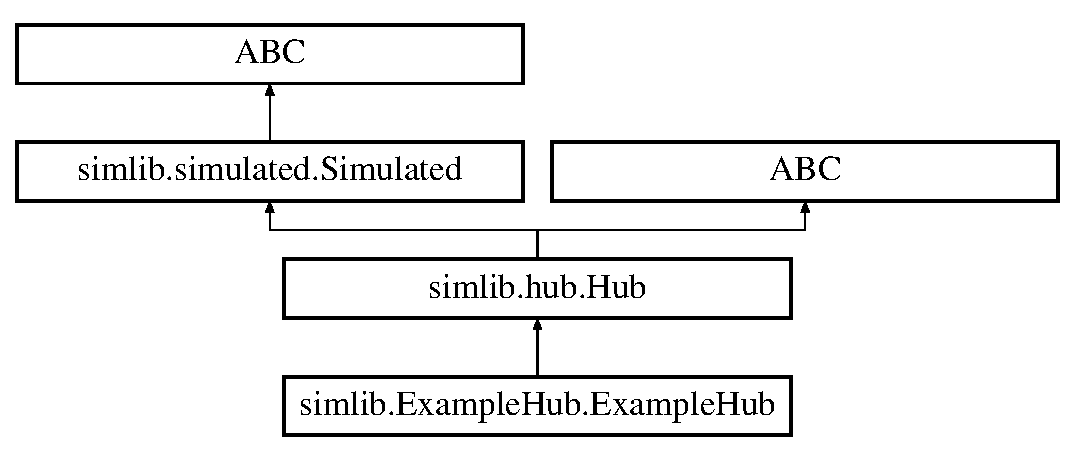
\includegraphics[height=4.000000cm]{classsimlib_1_1_example_hub_1_1_example_hub}
\end{center}
\end{figure}
\subsection*{Public Member Functions}
\begin{DoxyCompactItemize}
\item 
\mbox{\Hypertarget{classsimlib_1_1_example_hub_1_1_example_hub_a5d50debedd25fb1b15a868b42eb00bdc}\label{classsimlib_1_1_example_hub_1_1_example_hub_a5d50debedd25fb1b15a868b42eb00bdc}} 
def {\bfseries \+\_\+\+\_\+init\+\_\+\+\_\+} (self)
\item 
\mbox{\Hypertarget{classsimlib_1_1_example_hub_1_1_example_hub_a16fd9dc7c4e553dbb3e40cd75fda3b00}\label{classsimlib_1_1_example_hub_1_1_example_hub_a16fd9dc7c4e553dbb3e40cd75fda3b00}} 
def {\bfseries super\+Smart\+Trilateration\+Algorithm}
\item 
\mbox{\Hypertarget{classsimlib_1_1_example_hub_1_1_example_hub_acd64aed41178435d2195bd169fa86286}\label{classsimlib_1_1_example_hub_1_1_example_hub_acd64aed41178435d2195bd169fa86286}} 
def {\bfseries mainloop} (self)
\end{DoxyCompactItemize}
\subsection*{Public Attributes}
\begin{DoxyCompactItemize}
\item 
\mbox{\Hypertarget{classsimlib_1_1_example_hub_1_1_example_hub_a4c20526f36b9f6266f6686e2ed940042}\label{classsimlib_1_1_example_hub_1_1_example_hub_a4c20526f36b9f6266f6686e2ed940042}} 
{\bfseries algorithm}
\end{DoxyCompactItemize}


The documentation for this class was generated from the following file\+:\begin{DoxyCompactItemize}
\item 
src/simlib/Example\+Hub.\+py\end{DoxyCompactItemize}

\hypertarget{classsimlib_1_1hub_1_1_hub}{}\section{simlib.\+hub.\+Hub Class Reference}
\label{classsimlib_1_1hub_1_1_hub}\index{simlib.\+hub.\+Hub@{simlib.\+hub.\+Hub}}
Inheritance diagram for simlib.\+hub.\+Hub\+:\begin{figure}[H]
\begin{center}
\leavevmode
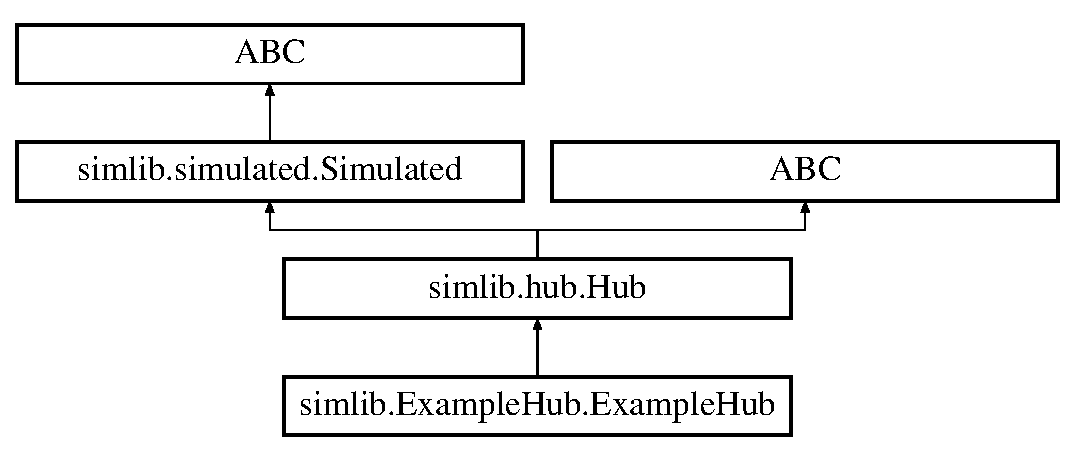
\includegraphics[height=3.000000cm]{classsimlib_1_1hub_1_1_hub}
\end{center}
\end{figure}
\subsection*{Public Member Functions}
\begin{DoxyCompactItemize}
\item 
def \mbox{\hyperlink{classsimlib_1_1hub_1_1_hub_aef9d9e20c18f3529bc77a67785994a3d}{\+\_\+\+\_\+init\+\_\+\+\_\+}} (self, \mbox{\hyperlink{classsimlib_1_1hub_1_1_hub_aca8e342d4c6bc56b75d88e0c715f817c}{algorithm}})
\item 
def \mbox{\hyperlink{classsimlib_1_1hub_1_1_hub_aee3b45cd9600d3c35c92bdb4871de586}{set\+Time}}
\item 
def \mbox{\hyperlink{classsimlib_1_1hub_1_1_hub_a32d013c48e8bf89093c30a847ee7f3c7}{contains\+Anchor}}
\item 
def \mbox{\hyperlink{classsimlib_1_1hub_1_1_hub_abdae7847cfc28517804da006cb55ee65}{add\+Anchor}}
\item 
def \mbox{\hyperlink{classsimlib_1_1hub_1_1_hub_abdcb60d6386e88f57ae1f111aae00cf5}{remove\+Anchor}}
\item 
def \mbox{\hyperlink{classsimlib_1_1hub_1_1_hub_a2e1b1b852d6a72f8511a1a66c98f938e}{contains\+Node}}
\item 
def \mbox{\hyperlink{classsimlib_1_1hub_1_1_hub_a91fe6d6f8365496de31b2550129bd27b}{add\+Node}}
\item 
def \mbox{\hyperlink{classsimlib_1_1hub_1_1_hub_a8adca099b501b37519bc755d47b43c35}{remove\+Node}}
\item 
def \mbox{\hyperlink{classsimlib_1_1hub_1_1_hub_acce9179de32abdcd091534e2d00b9156}{reset\+Map}} (self)
\item 
def \mbox{\hyperlink{classsimlib_1_1hub_1_1_hub_a6c7bcdb32a543f23d91f6c9fb5a684d3}{map\+Distance}}
\item 
def \mbox{\hyperlink{classsimlib_1_1hub_1_1_hub_a1f9e992128dff4752b3890c7678cec22}{get\+Node\+Position}}
\item 
def \mbox{\hyperlink{classsimlib_1_1hub_1_1_hub_a50cb83deb0326428d75dc520789f61c8}{map\+Anchor\+And\+Node}}
\item 
def \mbox{\hyperlink{classsimlib_1_1hub_1_1_hub_a131d5401102438d428e04a4caa24bd68}{triliterate\+Node}}
\item 
def \mbox{\hyperlink{classsimlib_1_1hub_1_1_hub_ad30ddbad3c34c11f7a392217578e39ad}{generate\+Complete\+Map}} (self)
\item 
def \mbox{\hyperlink{classsimlib_1_1hub_1_1_hub_aa1690052a9b14a68a6dff3dba2d8103e}{add\+Action}}
\item 
def \mbox{\hyperlink{classsimlib_1_1hub_1_1_hub_a1ee175090ec7c5b49a7ce93fca78e4cc}{prepend\+Action}}
\item 
def \mbox{\hyperlink{classsimlib_1_1hub_1_1_hub_ae460fbee94cf90c0c9f7dbce6770c015}{mainloop}} ()
\end{DoxyCompactItemize}
\subsection*{Public Attributes}
\begin{DoxyCompactItemize}
\item 
\mbox{\hyperlink{classsimlib_1_1hub_1_1_hub_a7db7bfdb073f30c1743c759f80e7bee0}{time}}
\item 
\mbox{\hyperlink{classsimlib_1_1hub_1_1_hub_a0029749fffb5dea111be831a18180a01}{anchors}}
\item 
\mbox{\hyperlink{classsimlib_1_1hub_1_1_hub_a61a34379fa5ce06d05763918fa3c619d}{nodes}}
\item 
\mbox{\hyperlink{classsimlib_1_1hub_1_1_hub_a04337df384aca498eb332aa200675754}{map}}
\item 
\mbox{\hyperlink{classsimlib_1_1hub_1_1_hub_a6fde0d1ce43d4b1ad2b98413b157d650}{node\+Positions}}
\item 
\mbox{\hyperlink{classsimlib_1_1hub_1_1_hub_aca8e342d4c6bc56b75d88e0c715f817c}{algorithm}}
\end{DoxyCompactItemize}


\subsection{Constructor \& Destructor Documentation}
\mbox{\Hypertarget{classsimlib_1_1hub_1_1_hub_aef9d9e20c18f3529bc77a67785994a3d}\label{classsimlib_1_1hub_1_1_hub_aef9d9e20c18f3529bc77a67785994a3d}} 
\index{simlib\+::hub\+::\+Hub@{simlib\+::hub\+::\+Hub}!\+\_\+\+\_\+init\+\_\+\+\_\+@{\+\_\+\+\_\+init\+\_\+\+\_\+}}
\index{\+\_\+\+\_\+init\+\_\+\+\_\+@{\+\_\+\+\_\+init\+\_\+\+\_\+}!simlib\+::hub\+::\+Hub@{simlib\+::hub\+::\+Hub}}
\subsubsection{\texorpdfstring{\+\_\+\+\_\+init\+\_\+\+\_\+()}{\_\_init\_\_()}}
{\footnotesize\ttfamily def simlib.\+hub.\+Hub.\+\_\+\+\_\+init\+\_\+\+\_\+ (\begin{DoxyParamCaption}\item[{}]{self,  }\item[{}]{algorithm }\end{DoxyParamCaption})}



\subsection{Member Function Documentation}
\mbox{\Hypertarget{classsimlib_1_1hub_1_1_hub_aa1690052a9b14a68a6dff3dba2d8103e}\label{classsimlib_1_1hub_1_1_hub_aa1690052a9b14a68a6dff3dba2d8103e}} 
\index{simlib\+::hub\+::\+Hub@{simlib\+::hub\+::\+Hub}!add\+Action@{add\+Action}}
\index{add\+Action@{add\+Action}!simlib\+::hub\+::\+Hub@{simlib\+::hub\+::\+Hub}}
\subsubsection{\texorpdfstring{add\+Action()}{addAction()}}
{\footnotesize\ttfamily def simlib.\+hub.\+Hub.\+add\+Action (\begin{DoxyParamCaption}\item[{}]{self,  }\item[{}]{function }\end{DoxyParamCaption})}

\mbox{\Hypertarget{classsimlib_1_1hub_1_1_hub_abdae7847cfc28517804da006cb55ee65}\label{classsimlib_1_1hub_1_1_hub_abdae7847cfc28517804da006cb55ee65}} 
\index{simlib\+::hub\+::\+Hub@{simlib\+::hub\+::\+Hub}!add\+Anchor@{add\+Anchor}}
\index{add\+Anchor@{add\+Anchor}!simlib\+::hub\+::\+Hub@{simlib\+::hub\+::\+Hub}}
\subsubsection{\texorpdfstring{add\+Anchor()}{addAnchor()}}
{\footnotesize\ttfamily def simlib.\+hub.\+Hub.\+add\+Anchor (\begin{DoxyParamCaption}\item[{}]{self,  }\item[{}]{anchor }\end{DoxyParamCaption})}

\mbox{\Hypertarget{classsimlib_1_1hub_1_1_hub_a91fe6d6f8365496de31b2550129bd27b}\label{classsimlib_1_1hub_1_1_hub_a91fe6d6f8365496de31b2550129bd27b}} 
\index{simlib\+::hub\+::\+Hub@{simlib\+::hub\+::\+Hub}!add\+Node@{add\+Node}}
\index{add\+Node@{add\+Node}!simlib\+::hub\+::\+Hub@{simlib\+::hub\+::\+Hub}}
\subsubsection{\texorpdfstring{add\+Node()}{addNode()}}
{\footnotesize\ttfamily def simlib.\+hub.\+Hub.\+add\+Node (\begin{DoxyParamCaption}\item[{}]{self,  }\item[{}]{node }\end{DoxyParamCaption})}

\mbox{\Hypertarget{classsimlib_1_1hub_1_1_hub_a32d013c48e8bf89093c30a847ee7f3c7}\label{classsimlib_1_1hub_1_1_hub_a32d013c48e8bf89093c30a847ee7f3c7}} 
\index{simlib\+::hub\+::\+Hub@{simlib\+::hub\+::\+Hub}!contains\+Anchor@{contains\+Anchor}}
\index{contains\+Anchor@{contains\+Anchor}!simlib\+::hub\+::\+Hub@{simlib\+::hub\+::\+Hub}}
\subsubsection{\texorpdfstring{contains\+Anchor()}{containsAnchor()}}
{\footnotesize\ttfamily def simlib.\+hub.\+Hub.\+contains\+Anchor (\begin{DoxyParamCaption}\item[{}]{self,  }\item[{}]{anchor }\end{DoxyParamCaption})}

\mbox{\Hypertarget{classsimlib_1_1hub_1_1_hub_a2e1b1b852d6a72f8511a1a66c98f938e}\label{classsimlib_1_1hub_1_1_hub_a2e1b1b852d6a72f8511a1a66c98f938e}} 
\index{simlib\+::hub\+::\+Hub@{simlib\+::hub\+::\+Hub}!contains\+Node@{contains\+Node}}
\index{contains\+Node@{contains\+Node}!simlib\+::hub\+::\+Hub@{simlib\+::hub\+::\+Hub}}
\subsubsection{\texorpdfstring{contains\+Node()}{containsNode()}}
{\footnotesize\ttfamily def simlib.\+hub.\+Hub.\+contains\+Node (\begin{DoxyParamCaption}\item[{}]{self,  }\item[{}]{node }\end{DoxyParamCaption})}

\mbox{\Hypertarget{classsimlib_1_1hub_1_1_hub_ad30ddbad3c34c11f7a392217578e39ad}\label{classsimlib_1_1hub_1_1_hub_ad30ddbad3c34c11f7a392217578e39ad}} 
\index{simlib\+::hub\+::\+Hub@{simlib\+::hub\+::\+Hub}!generate\+Complete\+Map@{generate\+Complete\+Map}}
\index{generate\+Complete\+Map@{generate\+Complete\+Map}!simlib\+::hub\+::\+Hub@{simlib\+::hub\+::\+Hub}}
\subsubsection{\texorpdfstring{generate\+Complete\+Map()}{generateCompleteMap()}}
{\footnotesize\ttfamily def simlib.\+hub.\+Hub.\+generate\+Complete\+Map (\begin{DoxyParamCaption}\item[{}]{self }\end{DoxyParamCaption})}

\begin{DoxyVerb}Generates a complete map of anchors and nodes
\end{DoxyVerb}
 \mbox{\Hypertarget{classsimlib_1_1hub_1_1_hub_a1f9e992128dff4752b3890c7678cec22}\label{classsimlib_1_1hub_1_1_hub_a1f9e992128dff4752b3890c7678cec22}} 
\index{simlib\+::hub\+::\+Hub@{simlib\+::hub\+::\+Hub}!get\+Node\+Position@{get\+Node\+Position}}
\index{get\+Node\+Position@{get\+Node\+Position}!simlib\+::hub\+::\+Hub@{simlib\+::hub\+::\+Hub}}
\subsubsection{\texorpdfstring{get\+Node\+Position()}{getNodePosition()}}
{\footnotesize\ttfamily def simlib.\+hub.\+Hub.\+get\+Node\+Position (\begin{DoxyParamCaption}\item[{}]{self,  }\item[{}]{node }\end{DoxyParamCaption})}

\mbox{\Hypertarget{classsimlib_1_1hub_1_1_hub_ae460fbee94cf90c0c9f7dbce6770c015}\label{classsimlib_1_1hub_1_1_hub_ae460fbee94cf90c0c9f7dbce6770c015}} 
\index{simlib\+::hub\+::\+Hub@{simlib\+::hub\+::\+Hub}!mainloop@{mainloop}}
\index{mainloop@{mainloop}!simlib\+::hub\+::\+Hub@{simlib\+::hub\+::\+Hub}}
\subsubsection{\texorpdfstring{mainloop()}{mainloop()}}
{\footnotesize\ttfamily def simlib.\+hub.\+Hub.\+mainloop (\begin{DoxyParamCaption}{ }\end{DoxyParamCaption})}

\mbox{\Hypertarget{classsimlib_1_1hub_1_1_hub_a50cb83deb0326428d75dc520789f61c8}\label{classsimlib_1_1hub_1_1_hub_a50cb83deb0326428d75dc520789f61c8}} 
\index{simlib\+::hub\+::\+Hub@{simlib\+::hub\+::\+Hub}!map\+Anchor\+And\+Node@{map\+Anchor\+And\+Node}}
\index{map\+Anchor\+And\+Node@{map\+Anchor\+And\+Node}!simlib\+::hub\+::\+Hub@{simlib\+::hub\+::\+Hub}}
\subsubsection{\texorpdfstring{map\+Anchor\+And\+Node()}{mapAnchorAndNode()}}
{\footnotesize\ttfamily def simlib.\+hub.\+Hub.\+map\+Anchor\+And\+Node (\begin{DoxyParamCaption}\item[{}]{self,  }\item[{}]{args }\end{DoxyParamCaption})}

\mbox{\Hypertarget{classsimlib_1_1hub_1_1_hub_a6c7bcdb32a543f23d91f6c9fb5a684d3}\label{classsimlib_1_1hub_1_1_hub_a6c7bcdb32a543f23d91f6c9fb5a684d3}} 
\index{simlib\+::hub\+::\+Hub@{simlib\+::hub\+::\+Hub}!map\+Distance@{map\+Distance}}
\index{map\+Distance@{map\+Distance}!simlib\+::hub\+::\+Hub@{simlib\+::hub\+::\+Hub}}
\subsubsection{\texorpdfstring{map\+Distance()}{mapDistance()}}
{\footnotesize\ttfamily def simlib.\+hub.\+Hub.\+map\+Distance (\begin{DoxyParamCaption}\item[{}]{self,  }\item[{}]{x\+Val }\end{DoxyParamCaption})}

\mbox{\Hypertarget{classsimlib_1_1hub_1_1_hub_a1ee175090ec7c5b49a7ce93fca78e4cc}\label{classsimlib_1_1hub_1_1_hub_a1ee175090ec7c5b49a7ce93fca78e4cc}} 
\index{simlib\+::hub\+::\+Hub@{simlib\+::hub\+::\+Hub}!prepend\+Action@{prepend\+Action}}
\index{prepend\+Action@{prepend\+Action}!simlib\+::hub\+::\+Hub@{simlib\+::hub\+::\+Hub}}
\subsubsection{\texorpdfstring{prepend\+Action()}{prependAction()}}
{\footnotesize\ttfamily def simlib.\+hub.\+Hub.\+prepend\+Action (\begin{DoxyParamCaption}\item[{}]{self,  }\item[{}]{function }\end{DoxyParamCaption})}

\mbox{\Hypertarget{classsimlib_1_1hub_1_1_hub_abdcb60d6386e88f57ae1f111aae00cf5}\label{classsimlib_1_1hub_1_1_hub_abdcb60d6386e88f57ae1f111aae00cf5}} 
\index{simlib\+::hub\+::\+Hub@{simlib\+::hub\+::\+Hub}!remove\+Anchor@{remove\+Anchor}}
\index{remove\+Anchor@{remove\+Anchor}!simlib\+::hub\+::\+Hub@{simlib\+::hub\+::\+Hub}}
\subsubsection{\texorpdfstring{remove\+Anchor()}{removeAnchor()}}
{\footnotesize\ttfamily def simlib.\+hub.\+Hub.\+remove\+Anchor (\begin{DoxyParamCaption}\item[{}]{self,  }\item[{}]{anchor }\end{DoxyParamCaption})}

\mbox{\Hypertarget{classsimlib_1_1hub_1_1_hub_a8adca099b501b37519bc755d47b43c35}\label{classsimlib_1_1hub_1_1_hub_a8adca099b501b37519bc755d47b43c35}} 
\index{simlib\+::hub\+::\+Hub@{simlib\+::hub\+::\+Hub}!remove\+Node@{remove\+Node}}
\index{remove\+Node@{remove\+Node}!simlib\+::hub\+::\+Hub@{simlib\+::hub\+::\+Hub}}
\subsubsection{\texorpdfstring{remove\+Node()}{removeNode()}}
{\footnotesize\ttfamily def simlib.\+hub.\+Hub.\+remove\+Node (\begin{DoxyParamCaption}\item[{}]{self,  }\item[{}]{node }\end{DoxyParamCaption})}

\mbox{\Hypertarget{classsimlib_1_1hub_1_1_hub_acce9179de32abdcd091534e2d00b9156}\label{classsimlib_1_1hub_1_1_hub_acce9179de32abdcd091534e2d00b9156}} 
\index{simlib\+::hub\+::\+Hub@{simlib\+::hub\+::\+Hub}!reset\+Map@{reset\+Map}}
\index{reset\+Map@{reset\+Map}!simlib\+::hub\+::\+Hub@{simlib\+::hub\+::\+Hub}}
\subsubsection{\texorpdfstring{reset\+Map()}{resetMap()}}
{\footnotesize\ttfamily def simlib.\+hub.\+Hub.\+reset\+Map (\begin{DoxyParamCaption}\item[{}]{self }\end{DoxyParamCaption})}

\begin{DoxyVerb}Resets the map to [][] \end{DoxyVerb}
 \mbox{\Hypertarget{classsimlib_1_1hub_1_1_hub_aee3b45cd9600d3c35c92bdb4871de586}\label{classsimlib_1_1hub_1_1_hub_aee3b45cd9600d3c35c92bdb4871de586}} 
\index{simlib\+::hub\+::\+Hub@{simlib\+::hub\+::\+Hub}!set\+Time@{set\+Time}}
\index{set\+Time@{set\+Time}!simlib\+::hub\+::\+Hub@{simlib\+::hub\+::\+Hub}}
\subsubsection{\texorpdfstring{set\+Time()}{setTime()}}
{\footnotesize\ttfamily def simlib.\+hub.\+Hub.\+set\+Time (\begin{DoxyParamCaption}\item[{}]{time }\end{DoxyParamCaption})}

\mbox{\Hypertarget{classsimlib_1_1hub_1_1_hub_a131d5401102438d428e04a4caa24bd68}\label{classsimlib_1_1hub_1_1_hub_a131d5401102438d428e04a4caa24bd68}} 
\index{simlib\+::hub\+::\+Hub@{simlib\+::hub\+::\+Hub}!triliterate\+Node@{triliterate\+Node}}
\index{triliterate\+Node@{triliterate\+Node}!simlib\+::hub\+::\+Hub@{simlib\+::hub\+::\+Hub}}
\subsubsection{\texorpdfstring{triliterate\+Node()}{triliterateNode()}}
{\footnotesize\ttfamily def simlib.\+hub.\+Hub.\+triliterate\+Node (\begin{DoxyParamCaption}\item[{}]{node }\end{DoxyParamCaption})}



\subsection{Member Data Documentation}
\mbox{\Hypertarget{classsimlib_1_1hub_1_1_hub_aca8e342d4c6bc56b75d88e0c715f817c}\label{classsimlib_1_1hub_1_1_hub_aca8e342d4c6bc56b75d88e0c715f817c}} 
\index{simlib\+::hub\+::\+Hub@{simlib\+::hub\+::\+Hub}!algorithm@{algorithm}}
\index{algorithm@{algorithm}!simlib\+::hub\+::\+Hub@{simlib\+::hub\+::\+Hub}}
\subsubsection{\texorpdfstring{algorithm}{algorithm}}
{\footnotesize\ttfamily simlib.\+hub.\+Hub.\+algorithm}

\mbox{\Hypertarget{classsimlib_1_1hub_1_1_hub_a0029749fffb5dea111be831a18180a01}\label{classsimlib_1_1hub_1_1_hub_a0029749fffb5dea111be831a18180a01}} 
\index{simlib\+::hub\+::\+Hub@{simlib\+::hub\+::\+Hub}!anchors@{anchors}}
\index{anchors@{anchors}!simlib\+::hub\+::\+Hub@{simlib\+::hub\+::\+Hub}}
\subsubsection{\texorpdfstring{anchors}{anchors}}
{\footnotesize\ttfamily simlib.\+hub.\+Hub.\+anchors}

\mbox{\Hypertarget{classsimlib_1_1hub_1_1_hub_a04337df384aca498eb332aa200675754}\label{classsimlib_1_1hub_1_1_hub_a04337df384aca498eb332aa200675754}} 
\index{simlib\+::hub\+::\+Hub@{simlib\+::hub\+::\+Hub}!map@{map}}
\index{map@{map}!simlib\+::hub\+::\+Hub@{simlib\+::hub\+::\+Hub}}
\subsubsection{\texorpdfstring{map}{map}}
{\footnotesize\ttfamily simlib.\+hub.\+Hub.\+map}

\mbox{\Hypertarget{classsimlib_1_1hub_1_1_hub_a6fde0d1ce43d4b1ad2b98413b157d650}\label{classsimlib_1_1hub_1_1_hub_a6fde0d1ce43d4b1ad2b98413b157d650}} 
\index{simlib\+::hub\+::\+Hub@{simlib\+::hub\+::\+Hub}!node\+Positions@{node\+Positions}}
\index{node\+Positions@{node\+Positions}!simlib\+::hub\+::\+Hub@{simlib\+::hub\+::\+Hub}}
\subsubsection{\texorpdfstring{node\+Positions}{nodePositions}}
{\footnotesize\ttfamily simlib.\+hub.\+Hub.\+node\+Positions}

\mbox{\Hypertarget{classsimlib_1_1hub_1_1_hub_a61a34379fa5ce06d05763918fa3c619d}\label{classsimlib_1_1hub_1_1_hub_a61a34379fa5ce06d05763918fa3c619d}} 
\index{simlib\+::hub\+::\+Hub@{simlib\+::hub\+::\+Hub}!nodes@{nodes}}
\index{nodes@{nodes}!simlib\+::hub\+::\+Hub@{simlib\+::hub\+::\+Hub}}
\subsubsection{\texorpdfstring{nodes}{nodes}}
{\footnotesize\ttfamily simlib.\+hub.\+Hub.\+nodes}

\mbox{\Hypertarget{classsimlib_1_1hub_1_1_hub_a7db7bfdb073f30c1743c759f80e7bee0}\label{classsimlib_1_1hub_1_1_hub_a7db7bfdb073f30c1743c759f80e7bee0}} 
\index{simlib\+::hub\+::\+Hub@{simlib\+::hub\+::\+Hub}!time@{time}}
\index{time@{time}!simlib\+::hub\+::\+Hub@{simlib\+::hub\+::\+Hub}}
\subsubsection{\texorpdfstring{time}{time}}
{\footnotesize\ttfamily simlib.\+hub.\+Hub.\+time}



The documentation for this class was generated from the following file\+:\begin{DoxyCompactItemize}
\item 
\mbox{\hyperlink{hub_8py}{hub.\+py}}\end{DoxyCompactItemize}

\hypertarget{classsimlib_1_1archspec_1_1_my_subclass}{}\section{simlib.\+archspec.\+My\+Subclass Class Reference}
\label{classsimlib_1_1archspec_1_1_my_subclass}\index{simlib.\+archspec.\+My\+Subclass@{simlib.\+archspec.\+My\+Subclass}}
Inheritance diagram for simlib.\+archspec.\+My\+Subclass\+:\begin{figure}[H]
\begin{center}
\leavevmode
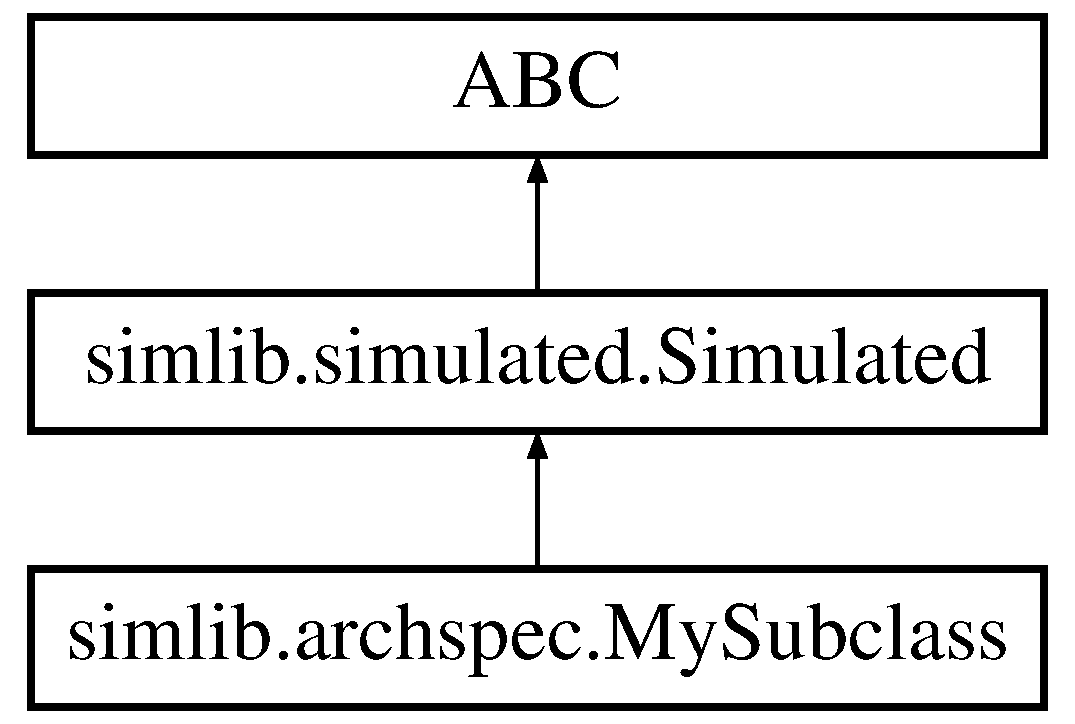
\includegraphics[height=3.000000cm]{classsimlib_1_1archspec_1_1_my_subclass}
\end{center}
\end{figure}
\subsection*{Additional Inherited Members}


The documentation for this class was generated from the following file\+:\begin{DoxyCompactItemize}
\item 
src/simlib/archspec.\+py\end{DoxyCompactItemize}

\hypertarget{classsimlib_1_1node_1_1_node}{}\section{simlib.\+node.\+Node Class Reference}
\label{classsimlib_1_1node_1_1_node}\index{simlib.\+node.\+Node@{simlib.\+node.\+Node}}
Inheritance diagram for simlib.\+node.\+Node\+:\begin{figure}[H]
\begin{center}
\leavevmode
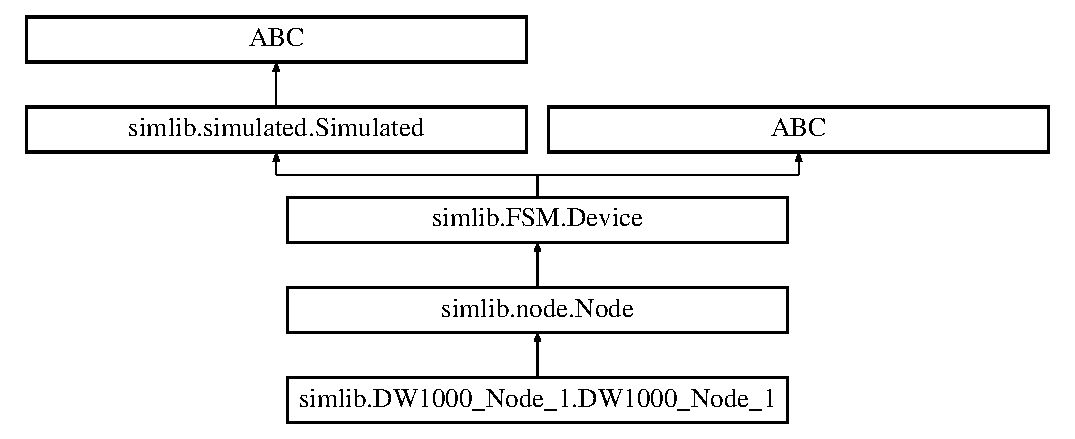
\includegraphics[height=4.000000cm]{classsimlib_1_1node_1_1_node}
\end{center}
\end{figure}
\subsection*{Public Member Functions}
\begin{DoxyCompactItemize}
\item 
def \mbox{\hyperlink{classsimlib_1_1node_1_1_node_ac6ef99e7e1c00c83ab001912a3d877b3}{\+\_\+\+\_\+init\+\_\+\+\_\+}}
\item 
def \mbox{\hyperlink{classsimlib_1_1node_1_1_node_a974a9b9f6f25605316255eb0e66e9f56}{set\+Time}}
\item 
def \mbox{\hyperlink{classsimlib_1_1node_1_1_node_a0bacc9e18647d14375eb93c26745d83c}{get\+ID}} ()
\item 
def \mbox{\hyperlink{classsimlib_1_1node_1_1_node_aa1c426997905e0825fdd529fe07f5538}{listen\+For\+Signal}} ()
\item 
def \mbox{\hyperlink{classsimlib_1_1node_1_1_node_a8c20a00c9d19ea5762c1388eaf232737}{add\+Action}}
\item 
def \mbox{\hyperlink{classsimlib_1_1node_1_1_node_a6ddb478f68f40125776533ea5c4f03b0}{prepend\+Action}}
\end{DoxyCompactItemize}
\subsection*{Public Attributes}
\begin{DoxyCompactItemize}
\item 
\mbox{\hyperlink{classsimlib_1_1node_1_1_node_a00cadc2f8f0b1641db5f678edb2ef080}{time}}
\item 
\mbox{\hyperlink{classsimlib_1_1node_1_1_node_af8798fcb88771789fce24e31e36b19af}{ID}}
\item 
\mbox{\hyperlink{classsimlib_1_1node_1_1_node_aca591a37f1bc0e27946fc32539b2218b}{x\+Pos}}
\item 
\mbox{\hyperlink{classsimlib_1_1node_1_1_node_a122d8d3c173fdd0463f01ef0cac3f1cc}{y\+Pos}}
\item 
\mbox{\hyperlink{classsimlib_1_1node_1_1_node_abb4fa2ca29a17b1fa2c3ab5dfc49f946}{z\+Pos}}
\item 
\mbox{\hyperlink{classsimlib_1_1node_1_1_node_a6ec4e0dd2c3ed5fb68cf34d91439df2f}{x\+Vel}}
\item 
\mbox{\hyperlink{classsimlib_1_1node_1_1_node_afad5609f2bb90cd489097775643b15e8}{y\+Vel}}
\item 
\mbox{\hyperlink{classsimlib_1_1node_1_1_node_ad6c09d6f475cfb8bb29455e4d03777dd}{z\+Vel}}
\item 
\mbox{\hyperlink{classsimlib_1_1node_1_1_node_a428c4962cfc4d2edbd87efcbd5271596}{signal\+List}}
\end{DoxyCompactItemize}


\subsection{Constructor \& Destructor Documentation}
\mbox{\Hypertarget{classsimlib_1_1node_1_1_node_ac6ef99e7e1c00c83ab001912a3d877b3}\label{classsimlib_1_1node_1_1_node_ac6ef99e7e1c00c83ab001912a3d877b3}} 
\index{simlib\+::node\+::\+Node@{simlib\+::node\+::\+Node}!\+\_\+\+\_\+init\+\_\+\+\_\+@{\+\_\+\+\_\+init\+\_\+\+\_\+}}
\index{\+\_\+\+\_\+init\+\_\+\+\_\+@{\+\_\+\+\_\+init\+\_\+\+\_\+}!simlib\+::node\+::\+Node@{simlib\+::node\+::\+Node}}
\subsubsection{\texorpdfstring{\+\_\+\+\_\+init\+\_\+\+\_\+()}{\_\_init\_\_()}}
{\footnotesize\ttfamily def simlib.\+node.\+Node.\+\_\+\+\_\+init\+\_\+\+\_\+ (\begin{DoxyParamCaption}\item[{}]{self,  }\item[{}]{ID }\end{DoxyParamCaption})}



\subsection{Member Function Documentation}
\mbox{\Hypertarget{classsimlib_1_1node_1_1_node_a8c20a00c9d19ea5762c1388eaf232737}\label{classsimlib_1_1node_1_1_node_a8c20a00c9d19ea5762c1388eaf232737}} 
\index{simlib\+::node\+::\+Node@{simlib\+::node\+::\+Node}!add\+Action@{add\+Action}}
\index{add\+Action@{add\+Action}!simlib\+::node\+::\+Node@{simlib\+::node\+::\+Node}}
\subsubsection{\texorpdfstring{add\+Action()}{addAction()}}
{\footnotesize\ttfamily def simlib.\+node.\+Node.\+add\+Action (\begin{DoxyParamCaption}\item[{}]{self,  }\item[{}]{function }\end{DoxyParamCaption})}

\mbox{\Hypertarget{classsimlib_1_1node_1_1_node_a0bacc9e18647d14375eb93c26745d83c}\label{classsimlib_1_1node_1_1_node_a0bacc9e18647d14375eb93c26745d83c}} 
\index{simlib\+::node\+::\+Node@{simlib\+::node\+::\+Node}!get\+ID@{get\+ID}}
\index{get\+ID@{get\+ID}!simlib\+::node\+::\+Node@{simlib\+::node\+::\+Node}}
\subsubsection{\texorpdfstring{get\+I\+D()}{getID()}}
{\footnotesize\ttfamily def simlib.\+node.\+Node.\+get\+ID (\begin{DoxyParamCaption}\item[{}]{int }\end{DoxyParamCaption})}

\mbox{\Hypertarget{classsimlib_1_1node_1_1_node_aa1c426997905e0825fdd529fe07f5538}\label{classsimlib_1_1node_1_1_node_aa1c426997905e0825fdd529fe07f5538}} 
\index{simlib\+::node\+::\+Node@{simlib\+::node\+::\+Node}!listen\+For\+Signal@{listen\+For\+Signal}}
\index{listen\+For\+Signal@{listen\+For\+Signal}!simlib\+::node\+::\+Node@{simlib\+::node\+::\+Node}}
\subsubsection{\texorpdfstring{listen\+For\+Signal()}{listenForSignal()}}
{\footnotesize\ttfamily def simlib.\+node.\+Node.\+listen\+For\+Signal (\begin{DoxyParamCaption}\item[{}]{int }\end{DoxyParamCaption})}

\begin{DoxyVerb}Searches to see if it is the target of any signals. Returns the sending ID
if a signal is found or 0 if no signal is found.
\end{DoxyVerb}
 \mbox{\Hypertarget{classsimlib_1_1node_1_1_node_a6ddb478f68f40125776533ea5c4f03b0}\label{classsimlib_1_1node_1_1_node_a6ddb478f68f40125776533ea5c4f03b0}} 
\index{simlib\+::node\+::\+Node@{simlib\+::node\+::\+Node}!prepend\+Action@{prepend\+Action}}
\index{prepend\+Action@{prepend\+Action}!simlib\+::node\+::\+Node@{simlib\+::node\+::\+Node}}
\subsubsection{\texorpdfstring{prepend\+Action()}{prependAction()}}
{\footnotesize\ttfamily def simlib.\+node.\+Node.\+prepend\+Action (\begin{DoxyParamCaption}\item[{}]{self,  }\item[{}]{function }\end{DoxyParamCaption})}

\mbox{\Hypertarget{classsimlib_1_1node_1_1_node_a974a9b9f6f25605316255eb0e66e9f56}\label{classsimlib_1_1node_1_1_node_a974a9b9f6f25605316255eb0e66e9f56}} 
\index{simlib\+::node\+::\+Node@{simlib\+::node\+::\+Node}!set\+Time@{set\+Time}}
\index{set\+Time@{set\+Time}!simlib\+::node\+::\+Node@{simlib\+::node\+::\+Node}}
\subsubsection{\texorpdfstring{set\+Time()}{setTime()}}
{\footnotesize\ttfamily def simlib.\+node.\+Node.\+set\+Time (\begin{DoxyParamCaption}\item[{}]{time }\end{DoxyParamCaption})}



\subsection{Member Data Documentation}
\mbox{\Hypertarget{classsimlib_1_1node_1_1_node_af8798fcb88771789fce24e31e36b19af}\label{classsimlib_1_1node_1_1_node_af8798fcb88771789fce24e31e36b19af}} 
\index{simlib\+::node\+::\+Node@{simlib\+::node\+::\+Node}!ID@{ID}}
\index{ID@{ID}!simlib\+::node\+::\+Node@{simlib\+::node\+::\+Node}}
\subsubsection{\texorpdfstring{ID}{ID}}
{\footnotesize\ttfamily simlib.\+node.\+Node.\+ID}

\mbox{\Hypertarget{classsimlib_1_1node_1_1_node_a428c4962cfc4d2edbd87efcbd5271596}\label{classsimlib_1_1node_1_1_node_a428c4962cfc4d2edbd87efcbd5271596}} 
\index{simlib\+::node\+::\+Node@{simlib\+::node\+::\+Node}!signal\+List@{signal\+List}}
\index{signal\+List@{signal\+List}!simlib\+::node\+::\+Node@{simlib\+::node\+::\+Node}}
\subsubsection{\texorpdfstring{signal\+List}{signalList}}
{\footnotesize\ttfamily simlib.\+node.\+Node.\+signal\+List}

\mbox{\Hypertarget{classsimlib_1_1node_1_1_node_a00cadc2f8f0b1641db5f678edb2ef080}\label{classsimlib_1_1node_1_1_node_a00cadc2f8f0b1641db5f678edb2ef080}} 
\index{simlib\+::node\+::\+Node@{simlib\+::node\+::\+Node}!time@{time}}
\index{time@{time}!simlib\+::node\+::\+Node@{simlib\+::node\+::\+Node}}
\subsubsection{\texorpdfstring{time}{time}}
{\footnotesize\ttfamily simlib.\+node.\+Node.\+time}

\mbox{\Hypertarget{classsimlib_1_1node_1_1_node_aca591a37f1bc0e27946fc32539b2218b}\label{classsimlib_1_1node_1_1_node_aca591a37f1bc0e27946fc32539b2218b}} 
\index{simlib\+::node\+::\+Node@{simlib\+::node\+::\+Node}!x\+Pos@{x\+Pos}}
\index{x\+Pos@{x\+Pos}!simlib\+::node\+::\+Node@{simlib\+::node\+::\+Node}}
\subsubsection{\texorpdfstring{x\+Pos}{xPos}}
{\footnotesize\ttfamily simlib.\+node.\+Node.\+x\+Pos}

\mbox{\Hypertarget{classsimlib_1_1node_1_1_node_a6ec4e0dd2c3ed5fb68cf34d91439df2f}\label{classsimlib_1_1node_1_1_node_a6ec4e0dd2c3ed5fb68cf34d91439df2f}} 
\index{simlib\+::node\+::\+Node@{simlib\+::node\+::\+Node}!x\+Vel@{x\+Vel}}
\index{x\+Vel@{x\+Vel}!simlib\+::node\+::\+Node@{simlib\+::node\+::\+Node}}
\subsubsection{\texorpdfstring{x\+Vel}{xVel}}
{\footnotesize\ttfamily simlib.\+node.\+Node.\+x\+Vel}

\mbox{\Hypertarget{classsimlib_1_1node_1_1_node_a122d8d3c173fdd0463f01ef0cac3f1cc}\label{classsimlib_1_1node_1_1_node_a122d8d3c173fdd0463f01ef0cac3f1cc}} 
\index{simlib\+::node\+::\+Node@{simlib\+::node\+::\+Node}!y\+Pos@{y\+Pos}}
\index{y\+Pos@{y\+Pos}!simlib\+::node\+::\+Node@{simlib\+::node\+::\+Node}}
\subsubsection{\texorpdfstring{y\+Pos}{yPos}}
{\footnotesize\ttfamily simlib.\+node.\+Node.\+y\+Pos}

\mbox{\Hypertarget{classsimlib_1_1node_1_1_node_afad5609f2bb90cd489097775643b15e8}\label{classsimlib_1_1node_1_1_node_afad5609f2bb90cd489097775643b15e8}} 
\index{simlib\+::node\+::\+Node@{simlib\+::node\+::\+Node}!y\+Vel@{y\+Vel}}
\index{y\+Vel@{y\+Vel}!simlib\+::node\+::\+Node@{simlib\+::node\+::\+Node}}
\subsubsection{\texorpdfstring{y\+Vel}{yVel}}
{\footnotesize\ttfamily simlib.\+node.\+Node.\+y\+Vel}

\mbox{\Hypertarget{classsimlib_1_1node_1_1_node_abb4fa2ca29a17b1fa2c3ab5dfc49f946}\label{classsimlib_1_1node_1_1_node_abb4fa2ca29a17b1fa2c3ab5dfc49f946}} 
\index{simlib\+::node\+::\+Node@{simlib\+::node\+::\+Node}!z\+Pos@{z\+Pos}}
\index{z\+Pos@{z\+Pos}!simlib\+::node\+::\+Node@{simlib\+::node\+::\+Node}}
\subsubsection{\texorpdfstring{z\+Pos}{zPos}}
{\footnotesize\ttfamily simlib.\+node.\+Node.\+z\+Pos}

\mbox{\Hypertarget{classsimlib_1_1node_1_1_node_ad6c09d6f475cfb8bb29455e4d03777dd}\label{classsimlib_1_1node_1_1_node_ad6c09d6f475cfb8bb29455e4d03777dd}} 
\index{simlib\+::node\+::\+Node@{simlib\+::node\+::\+Node}!z\+Vel@{z\+Vel}}
\index{z\+Vel@{z\+Vel}!simlib\+::node\+::\+Node@{simlib\+::node\+::\+Node}}
\subsubsection{\texorpdfstring{z\+Vel}{zVel}}
{\footnotesize\ttfamily simlib.\+node.\+Node.\+z\+Vel}



The documentation for this class was generated from the following file\+:\begin{DoxyCompactItemize}
\item 
\mbox{\hyperlink{node_8py}{node.\+py}}\end{DoxyCompactItemize}

\hypertarget{classsimlib_1_1simulated_1_1_simulated}{}\section{simlib.\+simulated.\+Simulated Class Reference}
\label{classsimlib_1_1simulated_1_1_simulated}\index{simlib.\+simulated.\+Simulated@{simlib.\+simulated.\+Simulated}}


Classes \#\#.  


Inheritance diagram for simlib.\+simulated.\+Simulated\+:\begin{figure}[H]
\begin{center}
\leavevmode
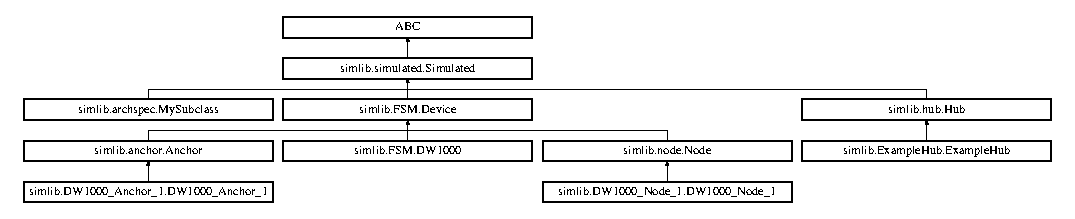
\includegraphics[height=4.000000cm]{classsimlib_1_1simulated_1_1_simulated}
\end{center}
\end{figure}
\subsection*{Public Member Functions}
\begin{DoxyCompactItemize}
\item 
def \mbox{\hyperlink{classsimlib_1_1simulated_1_1_simulated_aeb8d4e3ec653925db07aa4a13f128b0b}{\+\_\+\+\_\+init\+\_\+\+\_\+}} (self)
\item 
def \mbox{\hyperlink{classsimlib_1_1simulated_1_1_simulated_aef913462bcf40e1a2515fdc6f84ef8a4}{mainloop}}
\item 
def \mbox{\hyperlink{classsimlib_1_1simulated_1_1_simulated_a33d6b8f120ac2a359c8ea9b4a293967d}{run\+\_\+timestep}}
\end{DoxyCompactItemize}
\subsection*{Public Attributes}
\begin{DoxyCompactItemize}
\item 
\mbox{\hyperlink{classsimlib_1_1simulated_1_1_simulated_ae6258c72199dbdda082683c39a7dc336}{action\+Queue}}
\end{DoxyCompactItemize}


\subsection{Detailed Description}
Classes \#\#. 

\subsection{Constructor \& Destructor Documentation}
\mbox{\Hypertarget{classsimlib_1_1simulated_1_1_simulated_aeb8d4e3ec653925db07aa4a13f128b0b}\label{classsimlib_1_1simulated_1_1_simulated_aeb8d4e3ec653925db07aa4a13f128b0b}} 
\index{simlib\+::simulated\+::\+Simulated@{simlib\+::simulated\+::\+Simulated}!\+\_\+\+\_\+init\+\_\+\+\_\+@{\+\_\+\+\_\+init\+\_\+\+\_\+}}
\index{\+\_\+\+\_\+init\+\_\+\+\_\+@{\+\_\+\+\_\+init\+\_\+\+\_\+}!simlib\+::simulated\+::\+Simulated@{simlib\+::simulated\+::\+Simulated}}
\subsubsection{\texorpdfstring{\+\_\+\+\_\+init\+\_\+\+\_\+()}{\_\_init\_\_()}}
{\footnotesize\ttfamily def simlib.\+simulated.\+Simulated.\+\_\+\+\_\+init\+\_\+\+\_\+ (\begin{DoxyParamCaption}\item[{}]{self }\end{DoxyParamCaption})}



\subsection{Member Function Documentation}
\mbox{\Hypertarget{classsimlib_1_1simulated_1_1_simulated_aef913462bcf40e1a2515fdc6f84ef8a4}\label{classsimlib_1_1simulated_1_1_simulated_aef913462bcf40e1a2515fdc6f84ef8a4}} 
\index{simlib\+::simulated\+::\+Simulated@{simlib\+::simulated\+::\+Simulated}!mainloop@{mainloop}}
\index{mainloop@{mainloop}!simlib\+::simulated\+::\+Simulated@{simlib\+::simulated\+::\+Simulated}}
\subsubsection{\texorpdfstring{mainloop()}{mainloop()}}
{\footnotesize\ttfamily def simlib.\+simulated.\+Simulated.\+mainloop (\begin{DoxyParamCaption}\item[{}]{self,  }\item[{}]{simlist }\end{DoxyParamCaption})}

\mbox{\Hypertarget{classsimlib_1_1simulated_1_1_simulated_a33d6b8f120ac2a359c8ea9b4a293967d}\label{classsimlib_1_1simulated_1_1_simulated_a33d6b8f120ac2a359c8ea9b4a293967d}} 
\index{simlib\+::simulated\+::\+Simulated@{simlib\+::simulated\+::\+Simulated}!run\+\_\+timestep@{run\+\_\+timestep}}
\index{run\+\_\+timestep@{run\+\_\+timestep}!simlib\+::simulated\+::\+Simulated@{simlib\+::simulated\+::\+Simulated}}
\subsubsection{\texorpdfstring{run\+\_\+timestep()}{run\_timestep()}}
{\footnotesize\ttfamily def simlib.\+simulated.\+Simulated.\+run\+\_\+timestep (\begin{DoxyParamCaption}\item[{}]{self,  }\item[{}]{simlist }\end{DoxyParamCaption})}



\subsection{Member Data Documentation}
\mbox{\Hypertarget{classsimlib_1_1simulated_1_1_simulated_ae6258c72199dbdda082683c39a7dc336}\label{classsimlib_1_1simulated_1_1_simulated_ae6258c72199dbdda082683c39a7dc336}} 
\index{simlib\+::simulated\+::\+Simulated@{simlib\+::simulated\+::\+Simulated}!action\+Queue@{action\+Queue}}
\index{action\+Queue@{action\+Queue}!simlib\+::simulated\+::\+Simulated@{simlib\+::simulated\+::\+Simulated}}
\subsubsection{\texorpdfstring{action\+Queue}{actionQueue}}
{\footnotesize\ttfamily simlib.\+simulated.\+Simulated.\+action\+Queue}



The documentation for this class was generated from the following file\+:\begin{DoxyCompactItemize}
\item 
\mbox{\hyperlink{simulated_8py}{simulated.\+py}}\end{DoxyCompactItemize}

\hypertarget{classsimlib_1_1simulationenvironment_1_1_simulation_environment}{}\section{simlib.\+simulationenvironment.\+Simulation\+Environment Class Reference}
\label{classsimlib_1_1simulationenvironment_1_1_simulation_environment}\index{simlib.\+simulationenvironment.\+Simulation\+Environment@{simlib.\+simulationenvironment.\+Simulation\+Environment}}
\subsection*{Public Member Functions}
\begin{DoxyCompactItemize}
\item 
def \mbox{\hyperlink{classsimlib_1_1simulationenvironment_1_1_simulation_environment_a9523fb72f109de5e544efb6569f25b87}{\+\_\+\+\_\+init\+\_\+\+\_\+}} (self)
\item 
def \mbox{\hyperlink{classsimlib_1_1simulationenvironment_1_1_simulation_environment_a3663bc786f6efdb0fbeee270a89a5a09}{create\+Hub}}
\item 
def \mbox{\hyperlink{classsimlib_1_1simulationenvironment_1_1_simulation_environment_ae52e6b7ff377e9e19a42522cd556f810}{create\+Node}}
\item 
def \mbox{\hyperlink{classsimlib_1_1simulationenvironment_1_1_simulation_environment_a0ea1e1aed37d20521f1cd4a5fe45f304}{get\+Node\+By\+ID}}
\item 
def \mbox{\hyperlink{classsimlib_1_1simulationenvironment_1_1_simulation_environment_a300a94d4dcc67723f7a35c75bf17290d}{associate\+Node}}
\item 
def \mbox{\hyperlink{classsimlib_1_1simulationenvironment_1_1_simulation_environment_aeb0cf01f00d59cfdbd111e4ddae5c111}{dissassociate\+Node}}
\item 
def \mbox{\hyperlink{classsimlib_1_1simulationenvironment_1_1_simulation_environment_a5f7de813eb0a54424642ff1d57c6b0b2}{delete\+Node}}
\item 
def \mbox{\hyperlink{classsimlib_1_1simulationenvironment_1_1_simulation_environment_a2c100beae1b42193279b7eea874f05aa}{create\+Anchor}}
\item 
def \mbox{\hyperlink{classsimlib_1_1simulationenvironment_1_1_simulation_environment_a57dce9e31a624afdeb6185381cefbfd7}{get\+Anchor\+By\+ID}}
\item 
def \mbox{\hyperlink{classsimlib_1_1simulationenvironment_1_1_simulation_environment_a5c9ecc5861a006f3425c372141b419fe}{associate\+Anchor}}
\item 
def \mbox{\hyperlink{classsimlib_1_1simulationenvironment_1_1_simulation_environment_a8f5712a094eaac9c6101725d9bf7fa97}{dissassociate\+Anchor}}
\item 
def \mbox{\hyperlink{classsimlib_1_1simulationenvironment_1_1_simulation_environment_a54a6a5d3d58873223dec8396316ddf58}{delete\+Anchor}}
\item 
def \mbox{\hyperlink{classsimlib_1_1simulationenvironment_1_1_simulation_environment_ab842bfead4d18c821a01349409bc608a}{mainloop}} ()
\end{DoxyCompactItemize}
\subsection*{Public Attributes}
\begin{DoxyCompactItemize}
\item 
\mbox{\hyperlink{classsimlib_1_1simulationenvironment_1_1_simulation_environment_a81ac9426bfad791fb4a1ddaebace2545}{time}}
\item 
\mbox{\hyperlink{classsimlib_1_1simulationenvironment_1_1_simulation_environment_a04ccb1a4630854739716f8a50d971ac6}{hubs}}
\item 
\mbox{\hyperlink{classsimlib_1_1simulationenvironment_1_1_simulation_environment_a0f648c8fa4432c81ced68f989f1e56f0}{anchors}}
\item 
\mbox{\hyperlink{classsimlib_1_1simulationenvironment_1_1_simulation_environment_a8aa2d5276df2d1b1c328d9adf9ad18af}{nodes}}
\item 
\mbox{\hyperlink{classsimlib_1_1simulationenvironment_1_1_simulation_environment_aa4ded233ce51afb7b40a8cd62daa3ec7}{next\+ID}}
\item 
\mbox{\hyperlink{classsimlib_1_1simulationenvironment_1_1_simulation_environment_a27aced3ffaa804598044e5f73475c63f}{signal\+List}}
\end{DoxyCompactItemize}


\subsection{Constructor \& Destructor Documentation}
\mbox{\Hypertarget{classsimlib_1_1simulationenvironment_1_1_simulation_environment_a9523fb72f109de5e544efb6569f25b87}\label{classsimlib_1_1simulationenvironment_1_1_simulation_environment_a9523fb72f109de5e544efb6569f25b87}} 
\index{simlib\+::simulationenvironment\+::\+Simulation\+Environment@{simlib\+::simulationenvironment\+::\+Simulation\+Environment}!\+\_\+\+\_\+init\+\_\+\+\_\+@{\+\_\+\+\_\+init\+\_\+\+\_\+}}
\index{\+\_\+\+\_\+init\+\_\+\+\_\+@{\+\_\+\+\_\+init\+\_\+\+\_\+}!simlib\+::simulationenvironment\+::\+Simulation\+Environment@{simlib\+::simulationenvironment\+::\+Simulation\+Environment}}
\subsubsection{\texorpdfstring{\+\_\+\+\_\+init\+\_\+\+\_\+()}{\_\_init\_\_()}}
{\footnotesize\ttfamily def simlib.\+simulationenvironment.\+Simulation\+Environment.\+\_\+\+\_\+init\+\_\+\+\_\+ (\begin{DoxyParamCaption}\item[{}]{self }\end{DoxyParamCaption})}



\subsection{Member Function Documentation}
\mbox{\Hypertarget{classsimlib_1_1simulationenvironment_1_1_simulation_environment_a5c9ecc5861a006f3425c372141b419fe}\label{classsimlib_1_1simulationenvironment_1_1_simulation_environment_a5c9ecc5861a006f3425c372141b419fe}} 
\index{simlib\+::simulationenvironment\+::\+Simulation\+Environment@{simlib\+::simulationenvironment\+::\+Simulation\+Environment}!associate\+Anchor@{associate\+Anchor}}
\index{associate\+Anchor@{associate\+Anchor}!simlib\+::simulationenvironment\+::\+Simulation\+Environment@{simlib\+::simulationenvironment\+::\+Simulation\+Environment}}
\subsubsection{\texorpdfstring{associate\+Anchor()}{associateAnchor()}}
{\footnotesize\ttfamily def simlib.\+simulationenvironment.\+Simulation\+Environment.\+associate\+Anchor (\begin{DoxyParamCaption}\item[{}]{self,  }\item[{}]{hub }\end{DoxyParamCaption})}

\mbox{\Hypertarget{classsimlib_1_1simulationenvironment_1_1_simulation_environment_a300a94d4dcc67723f7a35c75bf17290d}\label{classsimlib_1_1simulationenvironment_1_1_simulation_environment_a300a94d4dcc67723f7a35c75bf17290d}} 
\index{simlib\+::simulationenvironment\+::\+Simulation\+Environment@{simlib\+::simulationenvironment\+::\+Simulation\+Environment}!associate\+Node@{associate\+Node}}
\index{associate\+Node@{associate\+Node}!simlib\+::simulationenvironment\+::\+Simulation\+Environment@{simlib\+::simulationenvironment\+::\+Simulation\+Environment}}
\subsubsection{\texorpdfstring{associate\+Node()}{associateNode()}}
{\footnotesize\ttfamily def simlib.\+simulationenvironment.\+Simulation\+Environment.\+associate\+Node (\begin{DoxyParamCaption}\item[{}]{self,  }\item[{}]{hub }\end{DoxyParamCaption})}

\mbox{\Hypertarget{classsimlib_1_1simulationenvironment_1_1_simulation_environment_a2c100beae1b42193279b7eea874f05aa}\label{classsimlib_1_1simulationenvironment_1_1_simulation_environment_a2c100beae1b42193279b7eea874f05aa}} 
\index{simlib\+::simulationenvironment\+::\+Simulation\+Environment@{simlib\+::simulationenvironment\+::\+Simulation\+Environment}!create\+Anchor@{create\+Anchor}}
\index{create\+Anchor@{create\+Anchor}!simlib\+::simulationenvironment\+::\+Simulation\+Environment@{simlib\+::simulationenvironment\+::\+Simulation\+Environment}}
\subsubsection{\texorpdfstring{create\+Anchor()}{createAnchor()}}
{\footnotesize\ttfamily def simlib.\+simulationenvironment.\+Simulation\+Environment.\+create\+Anchor (\begin{DoxyParamCaption}\item[{}]{self,  }\item[{}]{x\+Pos }\end{DoxyParamCaption})}

\mbox{\Hypertarget{classsimlib_1_1simulationenvironment_1_1_simulation_environment_a3663bc786f6efdb0fbeee270a89a5a09}\label{classsimlib_1_1simulationenvironment_1_1_simulation_environment_a3663bc786f6efdb0fbeee270a89a5a09}} 
\index{simlib\+::simulationenvironment\+::\+Simulation\+Environment@{simlib\+::simulationenvironment\+::\+Simulation\+Environment}!create\+Hub@{create\+Hub}}
\index{create\+Hub@{create\+Hub}!simlib\+::simulationenvironment\+::\+Simulation\+Environment@{simlib\+::simulationenvironment\+::\+Simulation\+Environment}}
\subsubsection{\texorpdfstring{create\+Hub()}{createHub()}}
{\footnotesize\ttfamily def simlib.\+simulationenvironment.\+Simulation\+Environment.\+create\+Hub (\begin{DoxyParamCaption}\item[{}]{self,  }\item[{}]{algorithm }\end{DoxyParamCaption})}

\mbox{\Hypertarget{classsimlib_1_1simulationenvironment_1_1_simulation_environment_ae52e6b7ff377e9e19a42522cd556f810}\label{classsimlib_1_1simulationenvironment_1_1_simulation_environment_ae52e6b7ff377e9e19a42522cd556f810}} 
\index{simlib\+::simulationenvironment\+::\+Simulation\+Environment@{simlib\+::simulationenvironment\+::\+Simulation\+Environment}!create\+Node@{create\+Node}}
\index{create\+Node@{create\+Node}!simlib\+::simulationenvironment\+::\+Simulation\+Environment@{simlib\+::simulationenvironment\+::\+Simulation\+Environment}}
\subsubsection{\texorpdfstring{create\+Node()}{createNode()}}
{\footnotesize\ttfamily def simlib.\+simulationenvironment.\+Simulation\+Environment.\+create\+Node (\begin{DoxyParamCaption}\item[{}]{self,  }\item[{}]{x\+Pos }\end{DoxyParamCaption})}

\mbox{\Hypertarget{classsimlib_1_1simulationenvironment_1_1_simulation_environment_a54a6a5d3d58873223dec8396316ddf58}\label{classsimlib_1_1simulationenvironment_1_1_simulation_environment_a54a6a5d3d58873223dec8396316ddf58}} 
\index{simlib\+::simulationenvironment\+::\+Simulation\+Environment@{simlib\+::simulationenvironment\+::\+Simulation\+Environment}!delete\+Anchor@{delete\+Anchor}}
\index{delete\+Anchor@{delete\+Anchor}!simlib\+::simulationenvironment\+::\+Simulation\+Environment@{simlib\+::simulationenvironment\+::\+Simulation\+Environment}}
\subsubsection{\texorpdfstring{delete\+Anchor()}{deleteAnchor()}}
{\footnotesize\ttfamily def simlib.\+simulationenvironment.\+Simulation\+Environment.\+delete\+Anchor (\begin{DoxyParamCaption}\item[{}]{self,  }\item[{}]{anchor }\end{DoxyParamCaption})}

\mbox{\Hypertarget{classsimlib_1_1simulationenvironment_1_1_simulation_environment_a5f7de813eb0a54424642ff1d57c6b0b2}\label{classsimlib_1_1simulationenvironment_1_1_simulation_environment_a5f7de813eb0a54424642ff1d57c6b0b2}} 
\index{simlib\+::simulationenvironment\+::\+Simulation\+Environment@{simlib\+::simulationenvironment\+::\+Simulation\+Environment}!delete\+Node@{delete\+Node}}
\index{delete\+Node@{delete\+Node}!simlib\+::simulationenvironment\+::\+Simulation\+Environment@{simlib\+::simulationenvironment\+::\+Simulation\+Environment}}
\subsubsection{\texorpdfstring{delete\+Node()}{deleteNode()}}
{\footnotesize\ttfamily def simlib.\+simulationenvironment.\+Simulation\+Environment.\+delete\+Node (\begin{DoxyParamCaption}\item[{}]{self,  }\item[{}]{node }\end{DoxyParamCaption})}

\mbox{\Hypertarget{classsimlib_1_1simulationenvironment_1_1_simulation_environment_a8f5712a094eaac9c6101725d9bf7fa97}\label{classsimlib_1_1simulationenvironment_1_1_simulation_environment_a8f5712a094eaac9c6101725d9bf7fa97}} 
\index{simlib\+::simulationenvironment\+::\+Simulation\+Environment@{simlib\+::simulationenvironment\+::\+Simulation\+Environment}!dissassociate\+Anchor@{dissassociate\+Anchor}}
\index{dissassociate\+Anchor@{dissassociate\+Anchor}!simlib\+::simulationenvironment\+::\+Simulation\+Environment@{simlib\+::simulationenvironment\+::\+Simulation\+Environment}}
\subsubsection{\texorpdfstring{dissassociate\+Anchor()}{dissassociateAnchor()}}
{\footnotesize\ttfamily def simlib.\+simulationenvironment.\+Simulation\+Environment.\+dissassociate\+Anchor (\begin{DoxyParamCaption}\item[{}]{hub }\end{DoxyParamCaption})}

\mbox{\Hypertarget{classsimlib_1_1simulationenvironment_1_1_simulation_environment_aeb0cf01f00d59cfdbd111e4ddae5c111}\label{classsimlib_1_1simulationenvironment_1_1_simulation_environment_aeb0cf01f00d59cfdbd111e4ddae5c111}} 
\index{simlib\+::simulationenvironment\+::\+Simulation\+Environment@{simlib\+::simulationenvironment\+::\+Simulation\+Environment}!dissassociate\+Node@{dissassociate\+Node}}
\index{dissassociate\+Node@{dissassociate\+Node}!simlib\+::simulationenvironment\+::\+Simulation\+Environment@{simlib\+::simulationenvironment\+::\+Simulation\+Environment}}
\subsubsection{\texorpdfstring{dissassociate\+Node()}{dissassociateNode()}}
{\footnotesize\ttfamily def simlib.\+simulationenvironment.\+Simulation\+Environment.\+dissassociate\+Node (\begin{DoxyParamCaption}\item[{}]{self,  }\item[{}]{hub }\end{DoxyParamCaption})}

\mbox{\Hypertarget{classsimlib_1_1simulationenvironment_1_1_simulation_environment_a57dce9e31a624afdeb6185381cefbfd7}\label{classsimlib_1_1simulationenvironment_1_1_simulation_environment_a57dce9e31a624afdeb6185381cefbfd7}} 
\index{simlib\+::simulationenvironment\+::\+Simulation\+Environment@{simlib\+::simulationenvironment\+::\+Simulation\+Environment}!get\+Anchor\+By\+ID@{get\+Anchor\+By\+ID}}
\index{get\+Anchor\+By\+ID@{get\+Anchor\+By\+ID}!simlib\+::simulationenvironment\+::\+Simulation\+Environment@{simlib\+::simulationenvironment\+::\+Simulation\+Environment}}
\subsubsection{\texorpdfstring{get\+Anchor\+By\+I\+D()}{getAnchorByID()}}
{\footnotesize\ttfamily def simlib.\+simulationenvironment.\+Simulation\+Environment.\+get\+Anchor\+By\+ID (\begin{DoxyParamCaption}\item[{}]{self,  }\item[{}]{ID }\end{DoxyParamCaption})}

\mbox{\Hypertarget{classsimlib_1_1simulationenvironment_1_1_simulation_environment_a0ea1e1aed37d20521f1cd4a5fe45f304}\label{classsimlib_1_1simulationenvironment_1_1_simulation_environment_a0ea1e1aed37d20521f1cd4a5fe45f304}} 
\index{simlib\+::simulationenvironment\+::\+Simulation\+Environment@{simlib\+::simulationenvironment\+::\+Simulation\+Environment}!get\+Node\+By\+ID@{get\+Node\+By\+ID}}
\index{get\+Node\+By\+ID@{get\+Node\+By\+ID}!simlib\+::simulationenvironment\+::\+Simulation\+Environment@{simlib\+::simulationenvironment\+::\+Simulation\+Environment}}
\subsubsection{\texorpdfstring{get\+Node\+By\+I\+D()}{getNodeByID()}}
{\footnotesize\ttfamily def simlib.\+simulationenvironment.\+Simulation\+Environment.\+get\+Node\+By\+ID (\begin{DoxyParamCaption}\item[{}]{self,  }\item[{}]{ID }\end{DoxyParamCaption})}

\mbox{\Hypertarget{classsimlib_1_1simulationenvironment_1_1_simulation_environment_ab842bfead4d18c821a01349409bc608a}\label{classsimlib_1_1simulationenvironment_1_1_simulation_environment_ab842bfead4d18c821a01349409bc608a}} 
\index{simlib\+::simulationenvironment\+::\+Simulation\+Environment@{simlib\+::simulationenvironment\+::\+Simulation\+Environment}!mainloop@{mainloop}}
\index{mainloop@{mainloop}!simlib\+::simulationenvironment\+::\+Simulation\+Environment@{simlib\+::simulationenvironment\+::\+Simulation\+Environment}}
\subsubsection{\texorpdfstring{mainloop()}{mainloop()}}
{\footnotesize\ttfamily def simlib.\+simulationenvironment.\+Simulation\+Environment.\+mainloop (\begin{DoxyParamCaption}{ }\end{DoxyParamCaption})}



\subsection{Member Data Documentation}
\mbox{\Hypertarget{classsimlib_1_1simulationenvironment_1_1_simulation_environment_a0f648c8fa4432c81ced68f989f1e56f0}\label{classsimlib_1_1simulationenvironment_1_1_simulation_environment_a0f648c8fa4432c81ced68f989f1e56f0}} 
\index{simlib\+::simulationenvironment\+::\+Simulation\+Environment@{simlib\+::simulationenvironment\+::\+Simulation\+Environment}!anchors@{anchors}}
\index{anchors@{anchors}!simlib\+::simulationenvironment\+::\+Simulation\+Environment@{simlib\+::simulationenvironment\+::\+Simulation\+Environment}}
\subsubsection{\texorpdfstring{anchors}{anchors}}
{\footnotesize\ttfamily simlib.\+simulationenvironment.\+Simulation\+Environment.\+anchors}

\mbox{\Hypertarget{classsimlib_1_1simulationenvironment_1_1_simulation_environment_a04ccb1a4630854739716f8a50d971ac6}\label{classsimlib_1_1simulationenvironment_1_1_simulation_environment_a04ccb1a4630854739716f8a50d971ac6}} 
\index{simlib\+::simulationenvironment\+::\+Simulation\+Environment@{simlib\+::simulationenvironment\+::\+Simulation\+Environment}!hubs@{hubs}}
\index{hubs@{hubs}!simlib\+::simulationenvironment\+::\+Simulation\+Environment@{simlib\+::simulationenvironment\+::\+Simulation\+Environment}}
\subsubsection{\texorpdfstring{hubs}{hubs}}
{\footnotesize\ttfamily simlib.\+simulationenvironment.\+Simulation\+Environment.\+hubs}

\mbox{\Hypertarget{classsimlib_1_1simulationenvironment_1_1_simulation_environment_aa4ded233ce51afb7b40a8cd62daa3ec7}\label{classsimlib_1_1simulationenvironment_1_1_simulation_environment_aa4ded233ce51afb7b40a8cd62daa3ec7}} 
\index{simlib\+::simulationenvironment\+::\+Simulation\+Environment@{simlib\+::simulationenvironment\+::\+Simulation\+Environment}!next\+ID@{next\+ID}}
\index{next\+ID@{next\+ID}!simlib\+::simulationenvironment\+::\+Simulation\+Environment@{simlib\+::simulationenvironment\+::\+Simulation\+Environment}}
\subsubsection{\texorpdfstring{next\+ID}{nextID}}
{\footnotesize\ttfamily simlib.\+simulationenvironment.\+Simulation\+Environment.\+next\+ID}

\mbox{\Hypertarget{classsimlib_1_1simulationenvironment_1_1_simulation_environment_a8aa2d5276df2d1b1c328d9adf9ad18af}\label{classsimlib_1_1simulationenvironment_1_1_simulation_environment_a8aa2d5276df2d1b1c328d9adf9ad18af}} 
\index{simlib\+::simulationenvironment\+::\+Simulation\+Environment@{simlib\+::simulationenvironment\+::\+Simulation\+Environment}!nodes@{nodes}}
\index{nodes@{nodes}!simlib\+::simulationenvironment\+::\+Simulation\+Environment@{simlib\+::simulationenvironment\+::\+Simulation\+Environment}}
\subsubsection{\texorpdfstring{nodes}{nodes}}
{\footnotesize\ttfamily simlib.\+simulationenvironment.\+Simulation\+Environment.\+nodes}

\mbox{\Hypertarget{classsimlib_1_1simulationenvironment_1_1_simulation_environment_a27aced3ffaa804598044e5f73475c63f}\label{classsimlib_1_1simulationenvironment_1_1_simulation_environment_a27aced3ffaa804598044e5f73475c63f}} 
\index{simlib\+::simulationenvironment\+::\+Simulation\+Environment@{simlib\+::simulationenvironment\+::\+Simulation\+Environment}!signal\+List@{signal\+List}}
\index{signal\+List@{signal\+List}!simlib\+::simulationenvironment\+::\+Simulation\+Environment@{simlib\+::simulationenvironment\+::\+Simulation\+Environment}}
\subsubsection{\texorpdfstring{signal\+List}{signalList}}
{\footnotesize\ttfamily simlib.\+simulationenvironment.\+Simulation\+Environment.\+signal\+List}

\mbox{\Hypertarget{classsimlib_1_1simulationenvironment_1_1_simulation_environment_a81ac9426bfad791fb4a1ddaebace2545}\label{classsimlib_1_1simulationenvironment_1_1_simulation_environment_a81ac9426bfad791fb4a1ddaebace2545}} 
\index{simlib\+::simulationenvironment\+::\+Simulation\+Environment@{simlib\+::simulationenvironment\+::\+Simulation\+Environment}!time@{time}}
\index{time@{time}!simlib\+::simulationenvironment\+::\+Simulation\+Environment@{simlib\+::simulationenvironment\+::\+Simulation\+Environment}}
\subsubsection{\texorpdfstring{time}{time}}
{\footnotesize\ttfamily simlib.\+simulationenvironment.\+Simulation\+Environment.\+time}



The documentation for this class was generated from the following file\+:\begin{DoxyCompactItemize}
\item 
\mbox{\hyperlink{simulationenvironment_8py}{simulationenvironment.\+py}}\end{DoxyCompactItemize}

\hypertarget{classsimlib_1_1_f_s_m_1_1_state}{}\section{simlib.\+F\+S\+M.\+State Class Reference}
\label{classsimlib_1_1_f_s_m_1_1_state}\index{simlib.\+F\+S\+M.\+State@{simlib.\+F\+S\+M.\+State}}
\subsection*{Public Member Functions}
\begin{DoxyCompactItemize}
\item 
def \mbox{\hyperlink{classsimlib_1_1_f_s_m_1_1_state_a29b361fb27793289b8e476b6fd927ae5}{\+\_\+\+\_\+init\+\_\+\+\_\+}}
\item 
def \mbox{\hyperlink{classsimlib_1_1_f_s_m_1_1_state_a92eddcb3c69993196174f4626ac01cb6}{get\+Param}}
\end{DoxyCompactItemize}
\subsection*{Public Attributes}
\begin{DoxyCompactItemize}
\item 
\mbox{\hyperlink{classsimlib_1_1_f_s_m_1_1_state_ad26863e22f2f1f410b06d09d118cf340}{physical\+\_\+data}}
\end{DoxyCompactItemize}


\subsection{Detailed Description}
\begin{DoxyVerb}Creates instance of a State for the device.
\end{DoxyVerb}
 

\subsection{Constructor \& Destructor Documentation}
\mbox{\Hypertarget{classsimlib_1_1_f_s_m_1_1_state_a29b361fb27793289b8e476b6fd927ae5}\label{classsimlib_1_1_f_s_m_1_1_state_a29b361fb27793289b8e476b6fd927ae5}} 
\index{simlib\+::\+F\+S\+M\+::\+State@{simlib\+::\+F\+S\+M\+::\+State}!\+\_\+\+\_\+init\+\_\+\+\_\+@{\+\_\+\+\_\+init\+\_\+\+\_\+}}
\index{\+\_\+\+\_\+init\+\_\+\+\_\+@{\+\_\+\+\_\+init\+\_\+\+\_\+}!simlib\+::\+F\+S\+M\+::\+State@{simlib\+::\+F\+S\+M\+::\+State}}
\subsubsection{\texorpdfstring{\+\_\+\+\_\+init\+\_\+\+\_\+()}{\_\_init\_\_()}}
{\footnotesize\ttfamily def simlib.\+F\+S\+M.\+State.\+\_\+\+\_\+init\+\_\+\+\_\+ (\begin{DoxyParamCaption}\item[{}]{self,  }\item[{}]{physical\+\_\+data }\end{DoxyParamCaption})}



\subsection{Member Function Documentation}
\mbox{\Hypertarget{classsimlib_1_1_f_s_m_1_1_state_a92eddcb3c69993196174f4626ac01cb6}\label{classsimlib_1_1_f_s_m_1_1_state_a92eddcb3c69993196174f4626ac01cb6}} 
\index{simlib\+::\+F\+S\+M\+::\+State@{simlib\+::\+F\+S\+M\+::\+State}!get\+Param@{get\+Param}}
\index{get\+Param@{get\+Param}!simlib\+::\+F\+S\+M\+::\+State@{simlib\+::\+F\+S\+M\+::\+State}}
\subsubsection{\texorpdfstring{get\+Param()}{getParam()}}
{\footnotesize\ttfamily def simlib.\+F\+S\+M.\+State.\+get\+Param (\begin{DoxyParamCaption}\item[{}]{self,  }\item[{}]{param }\end{DoxyParamCaption})}



\subsection{Member Data Documentation}
\mbox{\Hypertarget{classsimlib_1_1_f_s_m_1_1_state_ad26863e22f2f1f410b06d09d118cf340}\label{classsimlib_1_1_f_s_m_1_1_state_ad26863e22f2f1f410b06d09d118cf340}} 
\index{simlib\+::\+F\+S\+M\+::\+State@{simlib\+::\+F\+S\+M\+::\+State}!physical\+\_\+data@{physical\+\_\+data}}
\index{physical\+\_\+data@{physical\+\_\+data}!simlib\+::\+F\+S\+M\+::\+State@{simlib\+::\+F\+S\+M\+::\+State}}
\subsubsection{\texorpdfstring{physical\+\_\+data}{physical\_data}}
{\footnotesize\ttfamily simlib.\+F\+S\+M.\+State.\+physical\+\_\+data}



The documentation for this class was generated from the following file\+:\begin{DoxyCompactItemize}
\item 
\mbox{\hyperlink{_f_s_m_8py}{F\+S\+M.\+py}}\end{DoxyCompactItemize}

%--- End generated contents ---

% Index
\backmatter
\newpage
\phantomsection
\clearemptydoublepage
\addcontentsline{toc}{chapter}{Index}
\printindex

\end{document}
